\documentclass[12pt]{jreport}
\usepackage{amsl_thesis}
\usepackage{tabularx}
\usepackage{comment}
\usepackage[dvipdfmx]{hyperref}
\usepackage{pxjahyper}
\usepackage{url}
%\usepackage{algorithm}
\usepackage{algorithm2e}
\usepackage{subcaption}
\makeatletter
\renewcommand{\@algocf@capt@plain}{above}% formerly {bottom}
\makeatother
\usepackage{algorithmic}
\usepackage[dvipdfmx]{graphicx}

\hypersetup{
	colorlinks=false,
	%bookmarks=true,
	bookmarksnumbered=true,
	pdfborder={0 0 0},
	bookmarkstype=toc
}

%%%%%%%%%%%%%%%%%%%%%%%%%%%%%%%%%%%%%%%%%%%%%%%%%%%%%%%%%%%%%%%%%%%%%%%%
\title{機械学習を利用したメッシュ地図生成と \\ ビジュアルローカリゼーション}
\author{河合 響}
\bachelar  % 卒業論文(B4用)
%\master % 修士論文(M2用)

\studentid{153R173013} % 学生番号
\gyear{2020} % 卒業年度
\date{2021年2月1日} % 論文提出日

%%%%%%%%%%%%%%%%%%%%%%%%%%%%%%%%%%%%%%%%%%%%%%%%%%%%%%%%%%%%%%%%%%%%%%%%

\begin{document}

\maketitle

\pagenumbering{roman}
%% 概要
\chapter*{概要}
\addcontentsline{toc}{chapter}{概要}{季節や天候,時間などによる環境変化に対してロバストなビジュアルローカリゼーションの達成はロボティクスにおいて重要な目標である.従来手法では機械学習を点群地図の生成と自己位置推定の両方に取り入れることでこれを達成してきた.しかし,二点間の間隔の大きい点群地図は視界外にある点が尤度算出の妨げになる,1つの点が持つ情報の重要度が上がりセンサーの誤差に弱くなるなど,尤度算出上の問題を抱えていた. \par 本研究ではこれらの問題解決のためにメッシュ地図を導入することで入り組んだ地形に対して頑強な尤度算出を可能とするビジュアルローカリゼーションを提案する.検証では点群地図とメッシュ地図での自己位置推定を行い,算出される尤度を比較することで本手法の有効性を示す.}


%% 目次
\tableofcontents
\listoffigures
\listoftables

\newpage
\pagenumbering{arabic}

%% 本文
%% 序論
\chapter{序論}
%%\cite{thrun2005probabilistic}
\section{はじめに}
 今日の日本は少子高齢化の影響による労働人口の減少に直面しており, その中でも運送業界やタクシー業界などでは深刻なドライバーの高齢化と働き手となる若者の不足に直面している. そのような状況下において自動運転技術の実用化に対する期待は非常に大きい. その中で自動運転の核となる技術である自己位置推定は古くから研究が進められてきた.自己位置推定には図\ref{fig:3D-PointCloud}のような点群データが得られるLiDAR(図\ref{fig:HDL-64E})やカメラ, GPSなどの機器が使用される. 近年ではカメラによる自己位置推定, 通称ビジュアルローカリゼーションを季節や時間などによる景色の光学的な変化に対して頑強にしようとする研究が盛んに行われている\cite{semantic_segmentation_in_snow}\cite{stenborg_2020}. 
\begin{figure}[htpb]
\begin{center}
\begin{tabular}{cc}
\begin{minipage}[t]{1.0\hsize}
\begin{center}
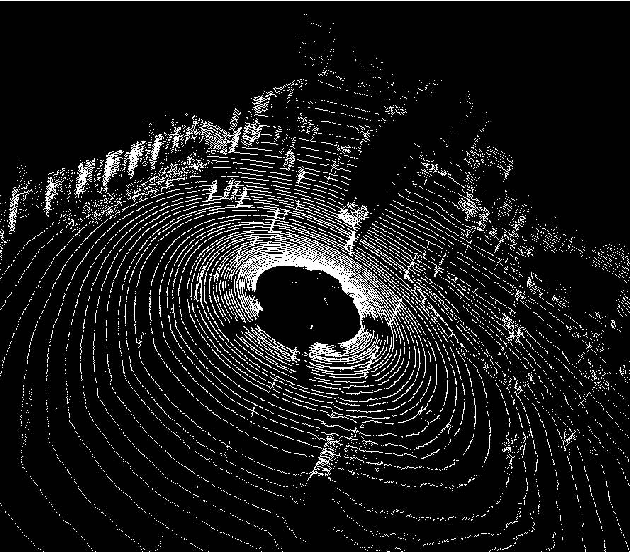
\includegraphics[width=5cm]{./picture/KITTI_pointcloud.png}
\caption{LiDARから得られた三次元点群}
\label{fig:3D-PointCloud}
\end{center}
\end{minipage} \\ \\
\begin{minipage}[t]{1.0\hsize}
\begin{center}
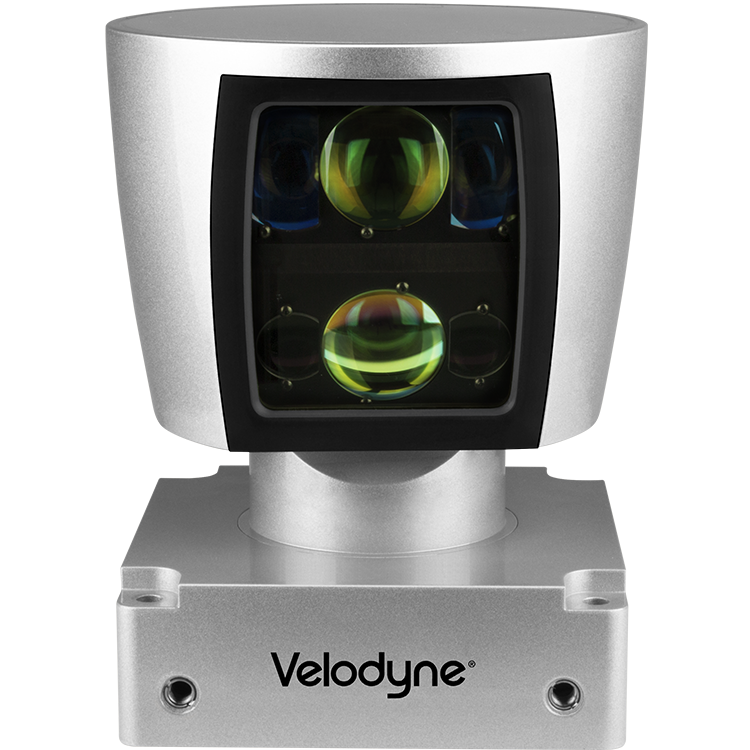
\includegraphics[width=5cm]{./picture/HDL64E.png}
\caption{Velodyne HDL-64E}
\label{fig:HDL-64E}
\end{center}
\end{minipage}
\end{tabular}
\end{center}
\end{figure}

\newpage
 
 \section{研究背景}
 ロボティクスにおいて自己位置推定は重要課題の一つである\cite{thrun2005probabilistic}. 自己位置推定の主なタスクはすでに構築された地図とロボットに搭載されたセンサからのデータを利用して確率統計学のアプローチから最もロボットが存在する確率の高い場所を算出することである。このときに使用されるセンサにはLiDARやカメラ, GPSなどが一般的でありその中でもカメラは比較的小型で安価であることから幅広い分野のロボットで使われている, ロボット掃除機の代表格でもあるiRobot社製のRoombaでもカメラによるビジュアルローカリゼーションを行っている\cite{Roomba_vSLAM}. \par ビジュアルローカリゼーションでは地図生成の際に抽出したエッジ\cite{Wuhan_Edge_Locali}やSIFTなどを始めとする特徴記述子等を三次元空間地図におけるランドマークとして配置し, ロボット搭載のカメラ画像から抽出した特徴量と比較することでロボット自身の位置を推定している\cite{vslam_survey}. 自動運転などを始めとするロボティクスの分野においてカメラから得られる情報は非常に使い勝手がよく, 先述のビジュアルローカリゼーションだけでなく人や車の検出など幅広く使われている\cite{DeepLab}. \par しかし, ビジュアルローカリゼーションにおいて頻繁に使用される特徴記述子には実用上で大きな問題が存在する. それは特徴記述子の抽出はコントラスト変化に対してはロバストであるものの, 昼と夜などの時間による景色の変化や季節変化による木や植物の色や日光のあたり方などの環境の変化には対応しきれないという点である\cite{Image_Recog_Kodansha}. さらにPedersonらの研究\cite{FeatureDescriptor}では一般的に使用されているSIFTやSURFなどの特徴記述子は光の状態に関して非常に敏感な反応を示すことが書かれている. 
これは特徴記述子の抽出が環境変化に対してロバストな設計ができたとしても, 地図とのマッチングの際に毎回同じ値で特徴子の抽出はできないため, 地図上の特徴点と比較するビジュアルローカリゼーションでは正確な尤度算出をする上で妨げになることを示唆している. したがってビジュアルローカリゼーションにおいて現在求められているものは季節や時間による環境変化に対してロバストなビジュアルローカリゼーションを実現すること, およびそれをより高い精度にすることである. \par この問題に対して, \ref{sec:related_work}節で述べる手法は環境変化に対して頑強な自己位置推定を実現した. しかし, その手法は複数の実用上の問題が存在する. 本研究ではそれらの問題を解決し実用的な自己位置推定手法を提案することを目的とする.
 
\begin{figure}[htbp]
\begin{center}
\begin{tabular}{c}
\begin{minipage}{0.7\hsize}
\begin{center}
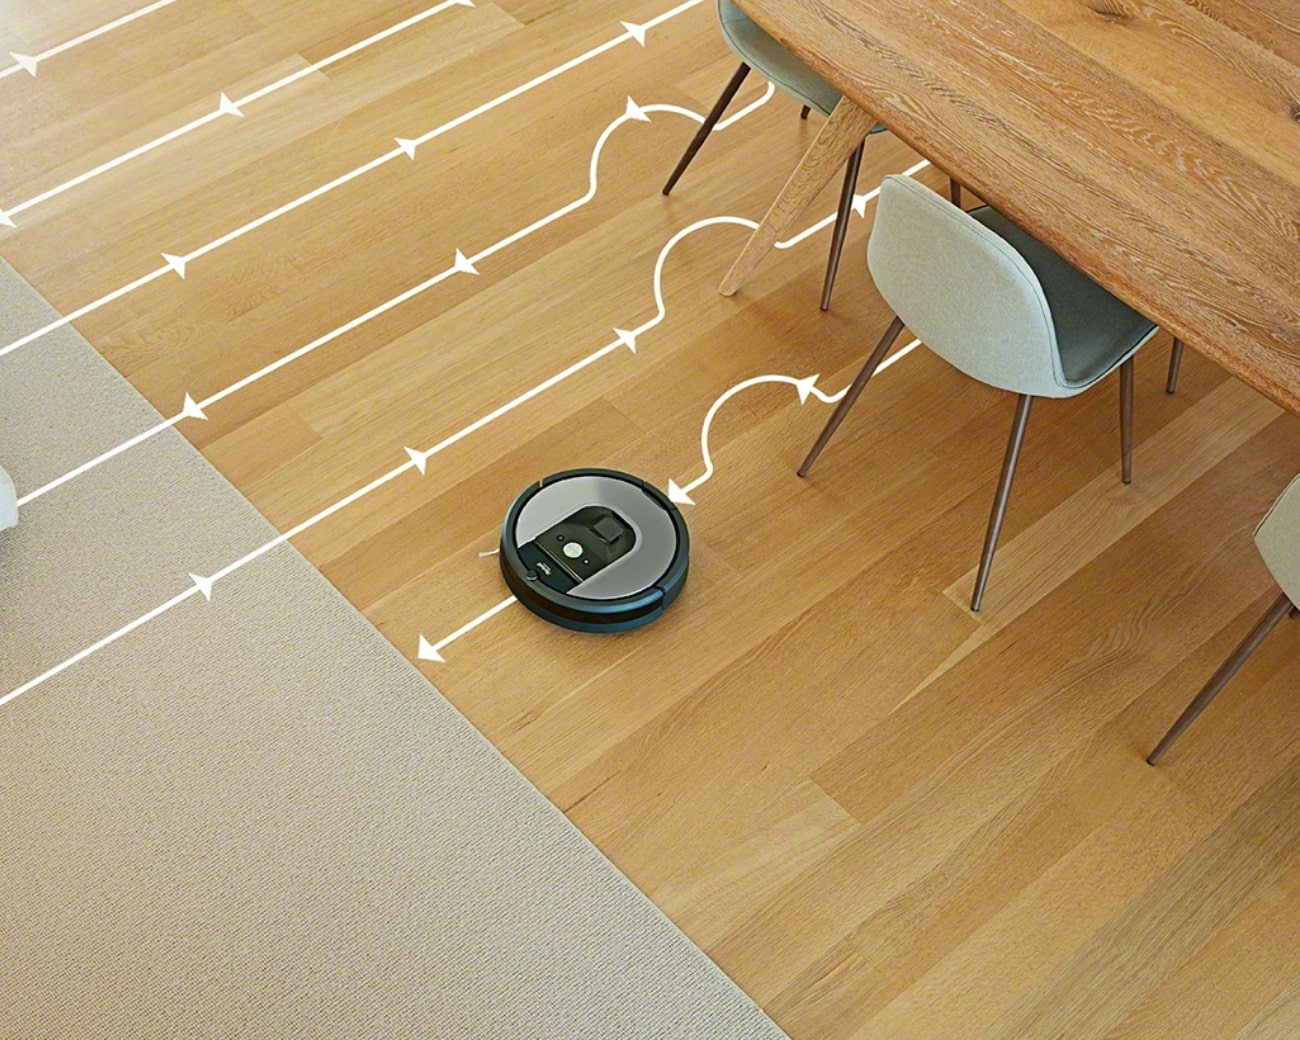
\includegraphics[width=10cm]{./picture/img-roomba.jpg}
\caption{iRobot社製 Roomba Series900}
\label{fig:Roomba}
\end{center}
\end{minipage}
\end{tabular}
\end{center}
\end{figure}

 \section{関連研究}\label{sec:related_work}
 先述の問題点に対して北海道大学の研究グループ\cite{semantic_segmentation_in_snow}とStenborgら\cite{semantic_point_localization}\cite{Toft_2018_ECCV}\cite{SattlerMTSPPO17}はそれぞれセマンティックセグメンテーションを地図生成とビジュアルローカリゼーションの両方で利用することで環境変化に対するロバスト性を実現しようとした. 機械学習を利用すれば季節の変化によって色や光の当たり方が変化したとしても学習時に同じ正解ラベルを与えることで図\ref{fig:ICNet}のようにセグメンテーションをする際には正しいクラスの出力結果が得られる. この特性を利用してStenborgらは図\ref{fig:SemanticPointLocalizationMap}のようにクラスごとに色分けされた三次元点群地図を生成, その地図の点とセグメンテーションしたカメラ画像をピクセル単位で比較することでビジュアルローカリゼーションを行った\cite{semantic_point_localization}. また, 地図にセマンティックな情報をもたせることで自己位置推定において地図上の木や建物などの物体が一種のランドマークとなる. これによってこれによって従来手法で用いられてきたQRコード\cite{QR_code_localization}や磁気マーカ\cite{jiki_marker_localization}などランドマークとなる人工物を設置する必要がないといったメリットが生まれる. \par この手法によって季節による特徴量抽出の変化の問題はある程度解決したが
2つの大きな問題が残った, 2つとも点群地図を使用することによるものである. 1つ目の問題点は点群地図はスパースな点で構成されているという問題であり, マッチングをする際には建物の裏側を構成する点群が図\ref{fig:Point_Cloud_Map}のように視界に入ってくるため住宅街など入り組んだ環境下ではピクセル単位で一致度を測定する時に尤度算出の妨げになる.2つ目はピクセル単位で点群地図と一致度を図る際に起こる問題点である. セグメンテーションされたカメラ画像と三次元のラベル付き点群地図をピクセル単位で比較する際, 点群地図だと少ない数の点でマッチングをする必要がある. これによって一つの点が持つ情報の重要度は相対的に上がり外乱などによるセグメンテーションの誤分類に脆弱になる. \par セマンティックな情報を地図生成と自己位置推定の両方に取り入れた研究はあまり多くなく, これらの問題に対して解決を図った研究は現時点で行われていない.
 
\begin{figure}[htbp]
\begin{tabular}{cc}
\begin{minipage}[t]{1.0\hsize}
\begin{center}
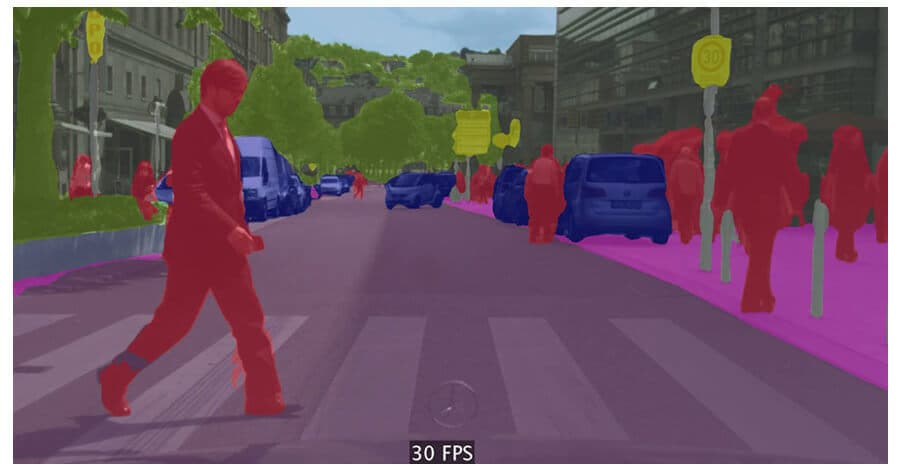
\includegraphics[width=14cm]{./picture/semseg.jpg}
\caption{セマンティックセグメンテーションの例}
\label{fig:ICNet}
\end{center}
\end{minipage} \\ \\
\begin{minipage}[t]{1.0\hsize}
\begin{center}
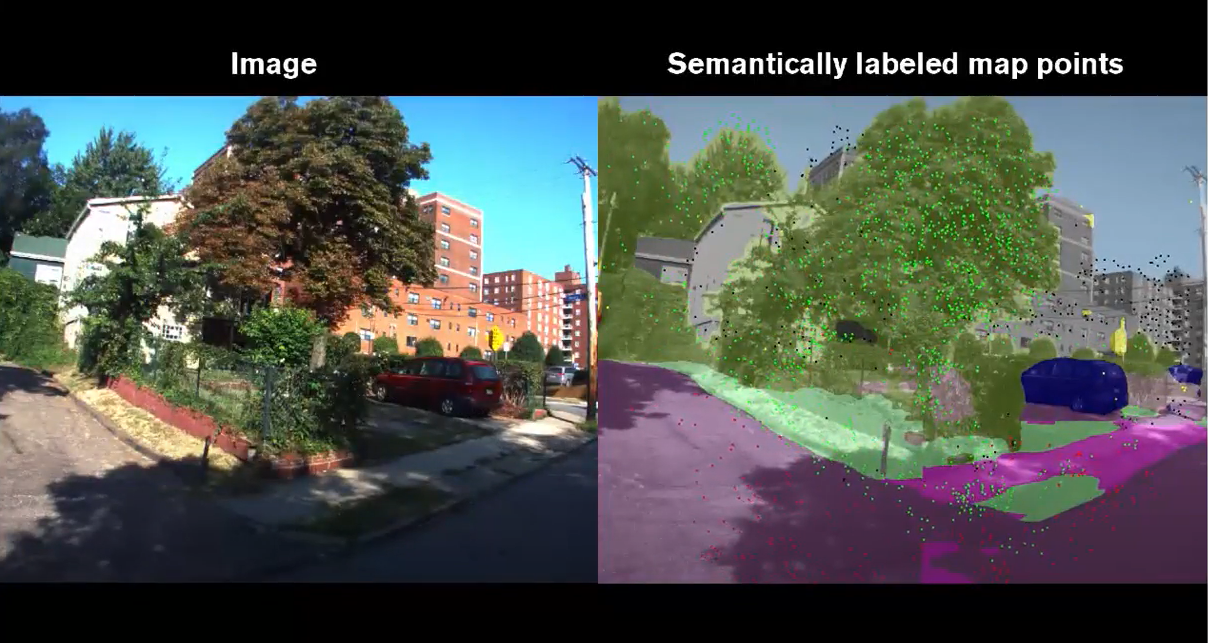
\includegraphics[width=14cm]{./picture/LongTermLocalization.png}
\caption{先行研究におけるカメラ画像(左), 及びラベル付けされた画像および点群地図(右)}
\label{fig:SemanticPointLocalizationMap}
\end{center}
\end{minipage} \\ \\
\begin{minipage}{1.0\hsize}
\begin{center}
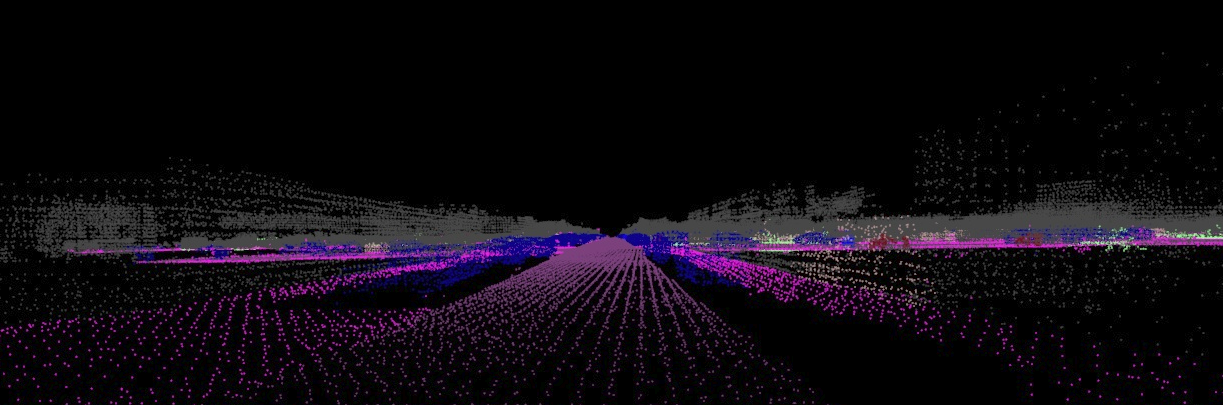
\includegraphics[width=14cm]{./picture/pc_map.png}
\caption{スパースな点群地図, 建物を構成する点群が手前の車を貫通して視界に入っている}
\label{fig:Point_Cloud_Map}
\end{center}
\end{minipage}
\end{tabular}
\end{figure}

\newpage
 
 \section{研究目的}
 本研究では先行研究で使われていたセマンティックな情報を持った点群地図をメッシュ地図に置き換えることで市街地などの入り組んだ地形に対して頑強な尤度算出を可能とするビジュアルローカリゼーションを提案する. また従来手法と「自己位置推定精度」, 及び「同じ状況下で一致しているとカウントされたピクセル数」の比較をすることで提案手法の有用性を示す.
%% 原理
\chapter{メッシュ地図を用いた自己位置推定}

\section{メッシュ地図での自己位置推定}
提案手法では, 自己位置推定の手法としてモンテカルロ自己位置推定\cite{MCL_paper}を用いた. モンテカルロ自己位置推定の数式などはAppendix \ref{app:monte_carlo}に示した. 提案手法における処理全体の流れとしてはAlg. \ref{alg:Overall}の通りである. このアルゴリズムの中で, (1)は\ref{sec:motion_update}節, (2)は\ref{sec:measurement_update}節, (3)は\ref{sec:estimate_current_pose}, (4)は\ref{sec:resampling}節でそれぞれ解説する.

\begin{algorithm}[htpb]
\SetAlgoLined
\caption{Semantic Mesh Localization Algorithm}
\label{alg:Overall}
 initialize particles $x_{0}$ and weights $w_{0}$\;
 \For{each time instance $t$}{
    acquire segmented image $y_{t}$\;
    motion update (1) \;
    \For{number of particles}{
        project 3D mesh map to 2D image in the view of particle $i$ as image $f_{t}^{i}$ \;
    }
    measurement update (2) \;
    normalize weights $w_{t}$\;
    estimate current pose $x_{t}$ (3)\;
    \If{resampling is needed}{
        resampling (4) \;
    }
 }
\end{algorithm}

%%%%ここからはコメントアウト
\begin{comment}
自己位置推定は最初の姿勢$x_{0}$,これまでの姿勢制御値$u_{1},u_{2}, ... ,u_{t}$, これまでのセンサ値のリスト$z_{1},z_{2}, ... ,z_{t}$からエージェントが現在の姿勢を更新する問題である. 自己位置推定を確率的な問題と扱うために現在の真の姿勢$x^{*}_{t}$に関する条件付き確率密度関数
\begin{equation}
    p_{t}(x|x_{0},u_{1},u_{2}, ... ,u_{t},z_{1},z_{2}, ... ,z_{t})
\end{equation}
を考える. $u_{1},u_{2}, ... ,u_{t}$を$u_{1:t}$, $z_{1},z_{2}, ... ,z_{t}$を$z_{1:t}$とおくと,
\begin{equation}
    p_{t}(x|x_{0}u_{1:t},z_{1:t})
\end{equation}
と表記できる. また, $u_{t}$を制御指令値と表記したがオドメトリやIMUなどのセンサを使った結果生じる移動量とすることもでき, ロボティクスにおいてはむしろそれが一般的である\cite[p108]{ueda_prob_robotics}. また移動量$u_{t}$については何らかの要因によって誤差が入っている時がある. 今回の実験では\ref{sec:dataset}節のとおり, 真値の移動量にガウス分布に従う誤差を加えた.\par 自己位置推定は時刻$t$における信念分布
\begin{equation}\label{eq:believe_total}
    b(t)=p_{t}(x|x_{0}u_{1:t},z_{1:t})
\end{equation}
を求めることに帰結する. \ref{eq:believe_total}をさらに分解すると入力である$x_{0},u_{1:t},z_{1:t}$, 状態遷移モデル$x_{t} \sim p(x|x_{t-1},u_{t})$, 観測モデル$z_{t} \sim p(z|x_{t})$に分解できる.\par 状態遷移モデル$x_{t} \sim p(x|x_{t-1},u_{t})$は信念分布$\hat{b}_{t}$として
\begin{equation}\label{eq:motion_update}
    \hat{b}(t)=p_{t}(x|x_{0},u_{1:t},z_{1:t-1})=p_{t}(x|x_{0},u_{1:t})
\end{equation}
と表現できる. $b_{t}$との違いはまだセンサ値$z_{t}$が反映されていない点である.この部分の詳細は\ref{sec:motion_update}節で詳しく述べる.\par 信念分布$b_{t}$は式\ref{eq:motion_update}の$\hat{b}_{t}$に\ref{sec:measurement_update}節で述べる観測モデルからの値$p(z_{t}|x)$を反映させることでできる. 式としては
\begin{equation}\label{eq:believe_equal}
    b_{t}(x)=\hat{b}_{t}(x|z_{t})=\frac{p(z_{t}|x)\hat{b}_{t}(x)}{p(z_{t})}=\eta p(z_{t}|x)\hat{b}_{t}(x)
\end{equation}
となる.
\end{comment}
%%%ここまでコメントアウト


\subsection{事前分布の更新}\label{sec:motion_update}
パーティクルフィルタにおいて事前分布の更新の目的は, 誤差を含むオドメトリやIMUなどの移動量に対してある確率分布に従ってパーティクルを分散させて信念分布$\hat{b}_{t}$の分布内に真の位置$x_{t}^{*}$をカバーすることである. パーティクル$i$において, 時刻$t-1$におけるパーティクルの位置$x_{t-1}^i$及び誤差を含む移動量$\Delta x_{t}$に対して事前分布の更新後の位置$\hat{x}_{t}^i$は
\begin{equation}\label{eq:motion_update_chapter}
    \hat{x}_{t}^i = x_{t-1}^i + \Delta x_{t} + \delta
\end{equation}
と表される. 今回の実験において, 式\ref{eq:motion_update_chapter}における$\delta$は平均$0$分散$\sigma^{2}$に従う正規分布$\mathcal{N}(0,\sigma^{2})$からドローできる.
\begin{equation}
    \delta \sim \mathcal{N}(0,\sigma^{2})
\end{equation}

\subsection{事後分布の更新}\label{sec:measurement_update}
パーティクルフィルタにおける事後分布の更新の目的は時刻$t$におけるパーティクルの尤度$w^{i}_{t}$を算出して後述する自己位置推定結果の算出やリサンプリングに役立てることである. \par セグメンテーションされたがカメラ画像を$y_{t}$パーティクルの位置$\hat{x}_{t}^{i}$から見た三次元メッシュ地図を二次元のRGB画像に変換したものを$f_{t}^{i}$として, 2つの画像を比較してセマンティックなクラスが一致したピクセルのみ抽出した画像を$d_{t}^{i}$とする. パーティクル$i$の尤度$w_{t}^{i}$は
\begin{equation}\label{eq:particle_likelihood}
    w_{t}^{i} = p(d_{t}^{i}|f_{t}^{i},y_{t},\hat{x}_{t}^{i},\mathcal{M})
\end{equation}
と表される. 式中の$\mathcal{M}$は三次元メッシュ地図を表している. \par 尤度算出のアルゴリズムはAlg. \ref{alg:calc_likelihood}の通りである. また, アルゴリズム中のsemantic scoreはピクセルのクラスごとに割り振られた値を出力する関数である. クラスごとの出力値は\ref{sec:env_appendix}節の表\ref{tab:likelihood_parameter}にある.

\begin{algorithm}[htpb]
 get segmented image as $y_{t}$ \;
 get mesh map image as $f_{t}^{i}$ \;
 $w^{i}_{t}$ = 0.0\;
 \If{The sizes of the $y_{t}$ and $f_{t}^{i}$ images match}{
    \For{$j=0$; $j<$size of image's height}{
        \For{$i=0$; $i<$size of image's width}{
            mesh class = semantic class of image $y_{t}$ at coordinate (i,j) \;
            image class = semantic class of image $f_{t}^{i}$ at coordinate(i,j) \;
            \If{mesh class == image class}{
                $w^{i}_{t}$ = $w^{i}_{t}$ + semantic score(image class) \;
            }
        }
    }
 }
 \Return $w^{i}_{t}$\;
 
 \caption{Calculating Likelihood Algorithms}
 \label{alg:calc_likelihood}
\end{algorithm}


\subsection{自己位置推定の結果の出力}\label{sec:estimate_current_pose}
\ref{sec:measurement_update}節において算出したパーティクル$w^{i}_{t}$を尤度が高い順に並べ替えて, 表\ref{tab:MCL_parameter}のAveragemumberの値$n$から上位$n$個のパーティクルのXYZ座標の平均を位置$x_{t}$のXYZ座標とした. 角度について, 本手法ではクオータニオンを角度表現に使っているが, クオータニオンは平均値の算出の計算が煩雑であるため\cite{Quaternion_average}最も尤度の高いパーティクルのクオータニオンを位置$x_{t}$の角度とした.

\subsection{リサンプリング}\label{sec:resampling}
 提案手法において用いられたリサンプリングの手法は系統サンプリング\cite{systematic_resampling_review}\cite{madow1944}と呼ばれるものである. パーティクル数を$n$, 各パーティクル$i$の尤度を$w_{t}^{i}$, 全パーティクルの尤度の合計を$\mathcal{W}$とすると系統サンプリングのアルゴリズムはAlg. \ref{alg:systematic_resampling_algorithm}の通りである.

\begin{algorithm}[htpb]
$w$ = empty vector\;
$acc = 0$\;
\For{$i=0$; $i<n$}{
    $acc = acc + w_{t}^{i}$\;
    $w$.append($acc$)\;
}
$step=\mathcal{W}/n$\;
$r \sim \mathcal{U}(0,step)$\;
$curpos=0$\;
$nw$ = empty vector\;
\While{size of $nw$ $<$ $\mathcal{W}$}{
    \eIf{$r<w[curpos]$}{
        $nw$.append($w_{t}^{curpos}$)\;
        $r=r+step$\;
        \If{$r>\mathcal{W}$}{
            $r=r-\mathcal{W}$\;
            $curpos=0$\;
        }
    }
    {
        $curpos+=1$\;
    }
}

\Return $nw$\;

 \caption{Systematic Resampling Algorithm}
 \label{alg:systematic_resampling_algorithm}
\end{algorithm}

%% Bonnetの解説
\section{セグメンテーション手法}
提案手法の有用性を示すための実験において, カメラ画像のセマンティックセグメンテーションの手法はBonnet\cite{milioto2019icra}を使用した. BonnetはGithub上で公開されているオープンソースのフレームワークであり, ROS環境下でリアルタイムなセグメンテーションをすることができるのが大きな特徴である. また, BonnetはGithub\cite{Bonnet_Github}から訓練済みのモデルをダウンロードすることが可能であり, CityScapes, Synthia\cite{RosCVPR16}, Persons\cite{Persons_Link}, Crop-Weed(CWC)\cite{chebrolu2017ijrr}の4つのデータセットから条件に応じた訓練済みデータを入手できる. 今回の実験ではCityScapesから学習した訓練済みデータを使用した.

\begin{figure}[htbp]
\begin{center}
\begin{tabular}{c}
\begin{minipage}{1.0\hsize}
\begin{center}
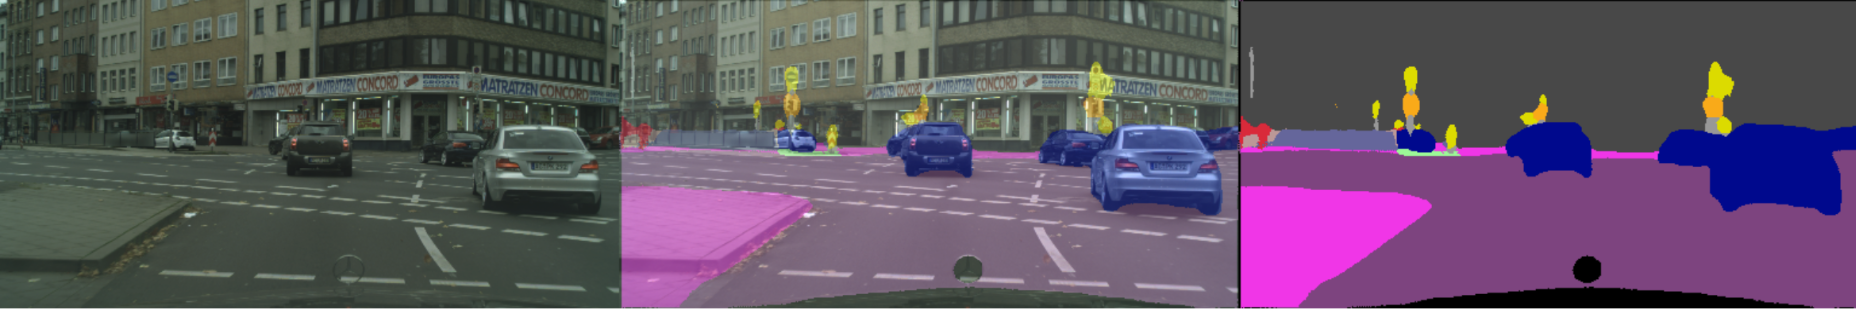
\includegraphics[width=14cm]{./picture/semantic_segmentation_bonnet.png}
\caption{Bonnetによるセマンティックセグメンテーション}
\label{fig:Bonnet}
\end{center}
\end{minipage}
\end{tabular}
\end{center}
\end{figure}

% Vexel Gridで点を間引いた間隔とかSLAMのやり方について書く
\section{メッシュ地図生成}
メッシュ地図のもととなる三次元点群地図の生成はデータセットのGround Truthを位置データを使用して行われた. そこからPCLのVoXelGrid Filter\cite{PCL_VexelGrid_Link}\cite{VoxelGrid_paper_1}\cite{VoxelGrid_paper_2}の機能を用いてクラスごとに異なる間隔で点群の間引きを行った.  メッシュ地図の生成は三次元点群地図からPCLのGreedyTriangulation\cite{Marton09ICRA}の機能を用いて作成した. 上記の通りの作成された点群地図は図\ref{fig:Point_Cloud_Map}, メッシュ地図は図\ref{fig:Mesh_Map}の通りである.

\begin{figure}[htbp]
\begin{center}
\begin{tabular}{c}
\begin{minipage}{1.0\hsize}
\begin{center}
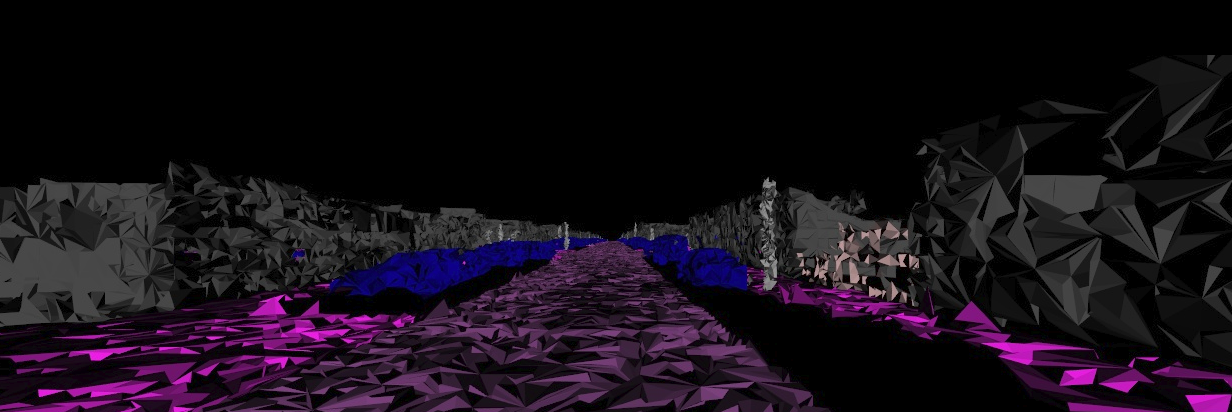
\includegraphics[width=14.5cm]{./picture/mesh_map.png}
\caption{メッシュ地図}
\label{fig:Mesh_Map}
\end{center}
\end{minipage}
\end{tabular}
\end{center}
\end{figure}

%\subsection{補足}

%% 実験環境
\chapter{実験環境}

\section{プログラム}
本実験で使用したプログラムは以下のサイト\cite{semantic_mesh_localization_link}にて公開している. また, 提案手法\cite{semantic_point_localization}はプログラムがインターネット上に公開されていないため論文内のアルゴリズムに従って作成した. 提案手法では画像のスキャンデータから三次元点群地図を生成しているが, 今回の実験においては\ref{sec:dataset}節で詳しく述べるデータセットから直接三次元点群を取得している部分が先行研究の論文内で述べられている実験環境と異なる.

%% PCの仕様
\section{PC}
今回実験では2台の性能の異なるPCを使用した. \ref{sec:result}節で述べる実験結果には動作時間の比較などを除いてPC1を使用したときの結果である. 以下の表\ref{tab:PC_spec}に使用したPCの性能を示す.

\begin{table}[htbp]
\begin{center}
\caption{PCスペック}
  \begin{tabular}{l c c}\hline
       &  PC1 & PC2 \\ \hline
    OS & Ubuntu20.04 LTS & Ubuntu18.04 LTS\\
    CPU & i9-10850K 10core 20thread 3.70GHz & i7-7700 4core 8thread 3.60GHz\\
    GPU & RTX2080Ti 8GB & GTX1060 3GB\\
    RAM & 32GB & 16GB\\ \hline
  \end{tabular}
  \label{tab:PC_spec}
\end{center}
\end{table}

\begin{comment}
\begin{table}[htbp]
\begin{center}
\caption{PC1スペック}
  \begin{tabular}{|l|c|}\hline
    OS & Ubuntu20.04 LTS \\ \hline
    NVIDIA Driver & 460.27.04 \\ \hline
    CPU & Intel Core i9-10850K 10コア 20スレッド 3.70GHz\\ \hline
    GPU & NVIDIA GeForce RTX2080Ti 8GB\\ \hline
    RAM & 32GB \\ \hline
  \end{tabular}
  \label{tab:PC1}
\end{center}
\end{table}

\begin{table}[htbp]
\begin{center}
\caption{PC2スペック}
  \begin{tabular}{|l|c|}\hline
    OS & Ubuntu18.04 LTS \\ \hline
    NVIDIA Driver & 460.27.04 \\ \hline
    CPU & Intel Core i7-7700 4 コア 8 スレッド 3.60GHz\\ \hline
    GPU & NVIDIA GeForce GTX1060 3GB\\ \hline
    RAM & 16GB \\ \hline
  \end{tabular}
  \label{tab:PC2}
\end{center}
\end{table}
\end{comment}


%% UbuntuでROSやTensorRT, PCLのどのバージョンを使いました的なことを書く
\section{ソフトウェア}\label{sec:software}
今回実験においてROSやOpenCV, PCLなどを中心としたソフトウェアを使用した. 表\ref{tab:software}に実験において使用したソフトウェアとそのバージョンを示す.
\begin{table}[htbp]
\begin{center}
\caption{実験に使用したソフトウェア}
  \begin{tabular}{l|c|c|l} \hline
    ソフトウェア名 & バージョン(PC1) & バージョン(PC2) & 備考 \\ \hline
    Robot Operation System & Noetic & Melodic & 以降"ROS"と表記する\\
    Point Cloud Library &1.8.1 & 1.8.1 & 以降"PCL"と表記する\\
    OpenCV & 3.2.0 & 3.2.0 & \\
    Visualization Toolkit & 9.0.1 & 9.0.1 & 以降"VTK"と表記する\\
    yaml-cpp & 0.6.2 & 0.5.2 & \\
    CUDA & 11.2 & 11.1 & \\
    nvinfer & 7.2.1-1 & 7.2.1-1 & \\
    Tensorflow & 2.3.1 & 2.3.1 & \\
    TensorRT & 7.2.1.6-1 & 7.2.1.6-1 & \\ \hline
  \end{tabular}
  \label{tab:software}
\end{center}
\end{table}

%% Semantic KITTIの解説
\section{データセット}\label{sec:dataset}
実験ではボン大学が公表しているSemantic KITTI dataset\cite{semantic_kitti_dataset_paper}\cite{semantic_kitti_dataset_link}を使用した. 本データセットはKITTI Visual Odometry Dataset\cite{Geiger2012CVPR}の点群データに車や建物などセマンティックなラベルを色として付与したPoint Segmentationの精度評価のためのデータセットである. 本データセットは点群にラベルの付いた11の学習用シークエンスとラベルの付いていない実験用の11のシークエンスからなるデータである. シークエンスの中には直線状の道路を10秒間走るだけといったものもあるが, 今回の実験ではそういったシークエンスは使用しない. 今回の実験で使用したシークエンスはsequence00, 02, 05, 08の4つである. それぞれのシークエンスの地図の全体像を図\ref{fig:sequence00}, \ref{fig:sequence02}, \ref{fig:sequence05}, \ref{fig:sequence08}に示す. \par 先行研究\cite{semantic_point_localization}では点群データの存在しないCityScapes Dataset\cite{CityScapes_paper}\cite{CityScapes_link}の画像データから三次元点群を生成して地図を作成していたが,本実験ではラベル付きのデータセットから直接地図を生成する. Semantic KITTI datasetから得られるデータは表\ref{tab:data_from_semantic_kitti}のとおりである. なお, Semantic KITTI datasetにはCityScapesやKITTI dataset\cite{KITTI_dataset_paper}のようにIMUやオドメトリのデータが存在しない. 自己位置推定を行うためには事前分布の更新のためにどちらか, もしくはその両方のデータが必要となる. このため実験では姿勢のGround Truthに正規分布に従う誤差を加えることでオドメトリを再現した. \par 今回ROS上で自己位置推定のためのプログラムを実行する上でこれらのデータセットをROSのbagデータに変換した. 変換に使用したプログラムはGithub上に公開してある\cite{semantickitti2bag}.

\begin{figure}[htbp]
 \begin{minipage}{0.5\hsize}
  \begin{center}
   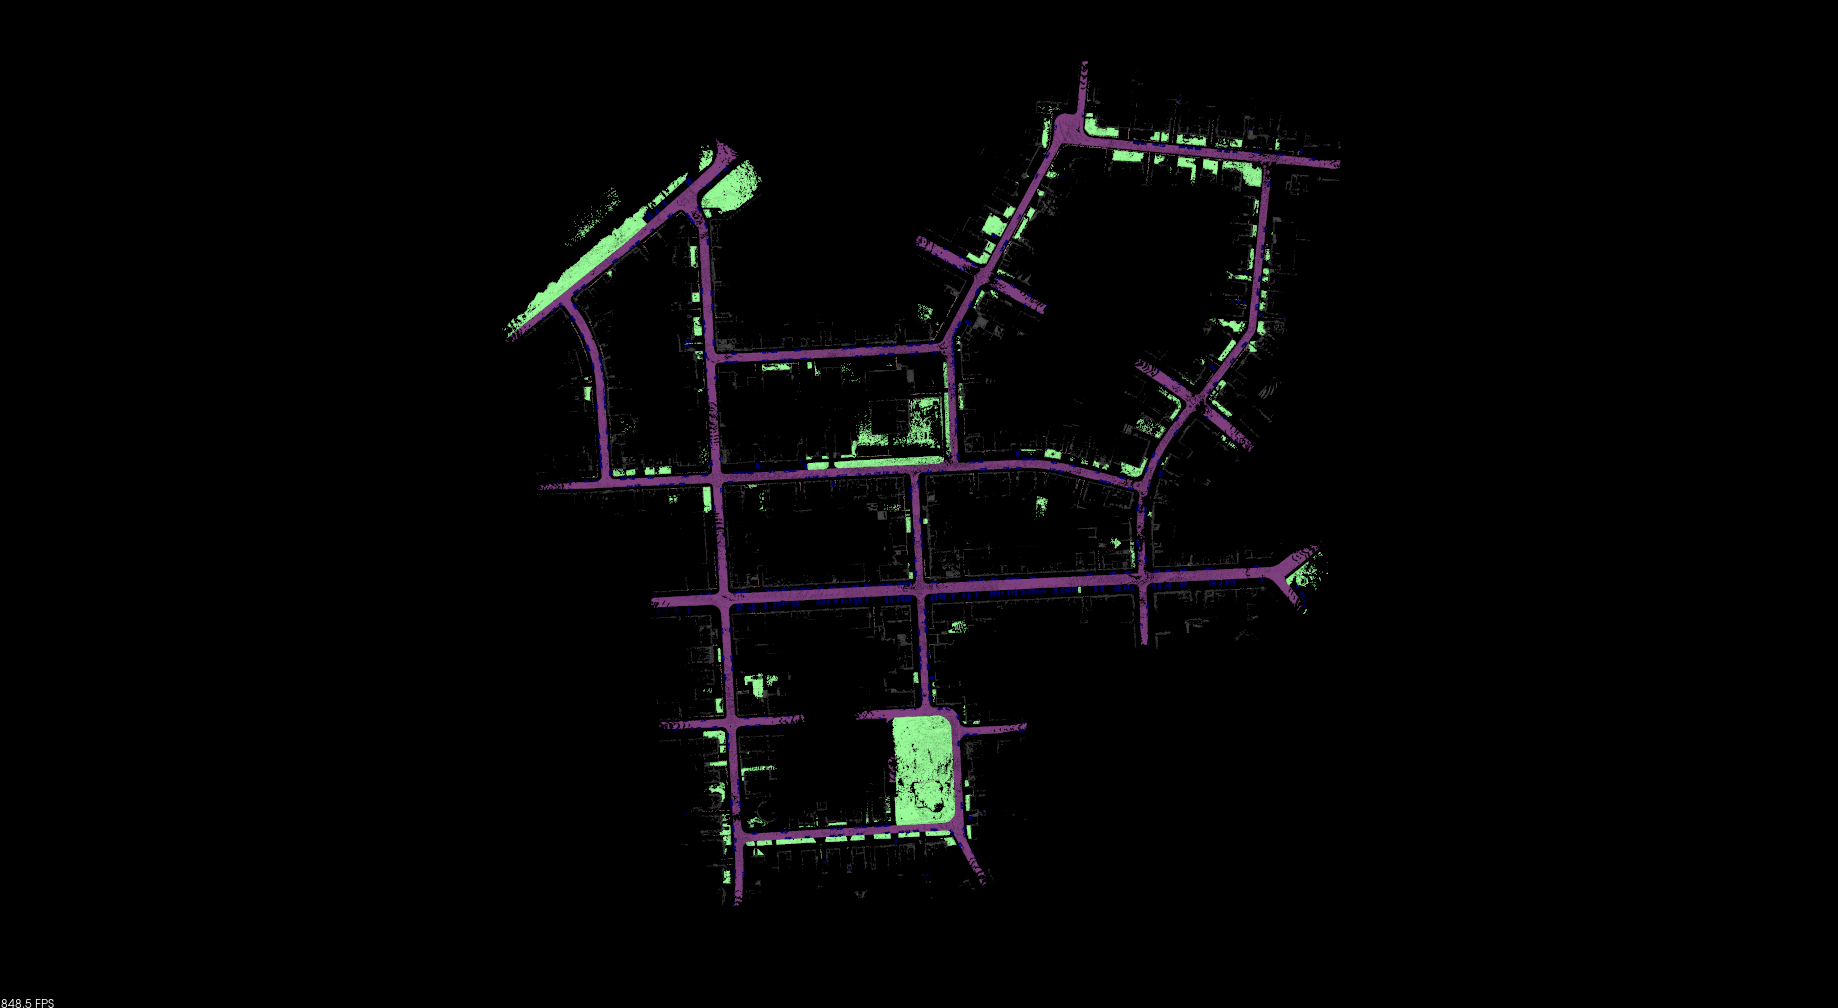
\includegraphics[width=75mm]{./picture/sequence00_map.png}
  \end{center}
  \caption{Sequence00}
  \label{fig:sequence00}
 \end{minipage}
 \begin{minipage}{0.5\hsize}
  \begin{center}
   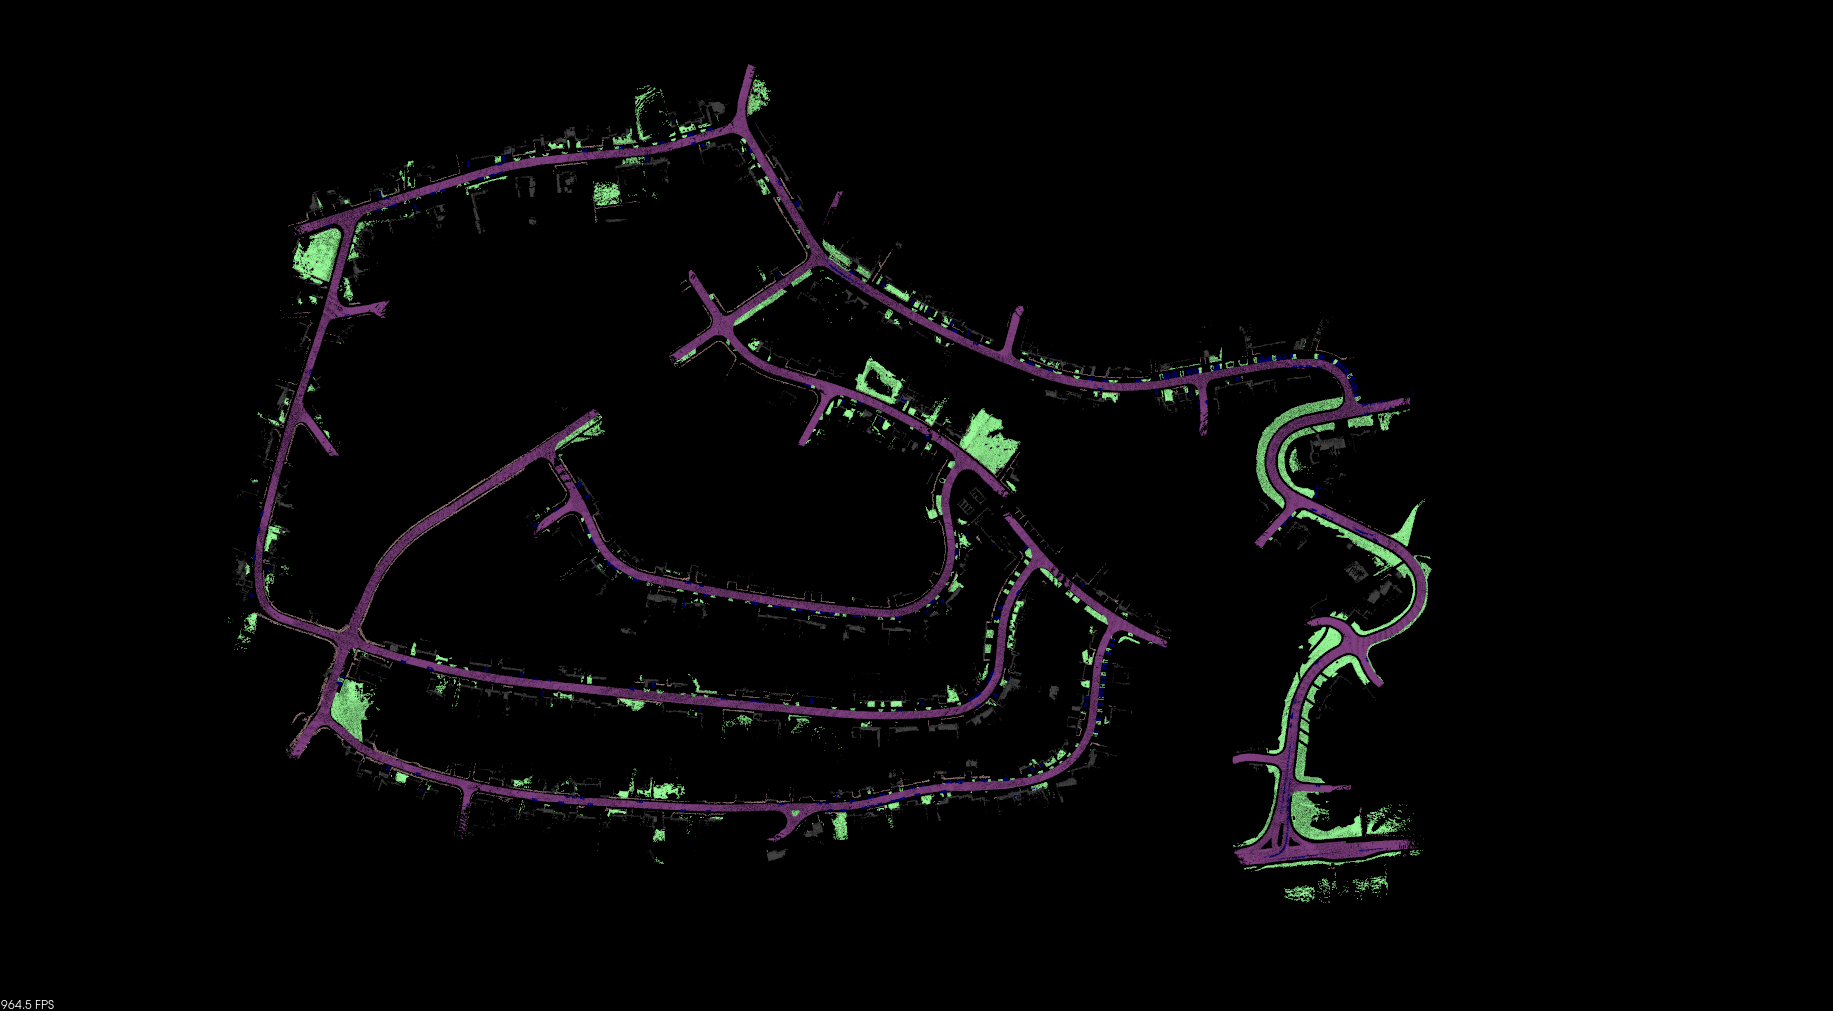
\includegraphics[width=75mm]{./picture/sequence02_map.png}
  \end{center}
  \caption{Sequence02}
  \label{fig:sequence02}
 \end{minipage} \\ \\ \\ \\
  \begin{minipage}{0.5\hsize}
  \begin{center}
   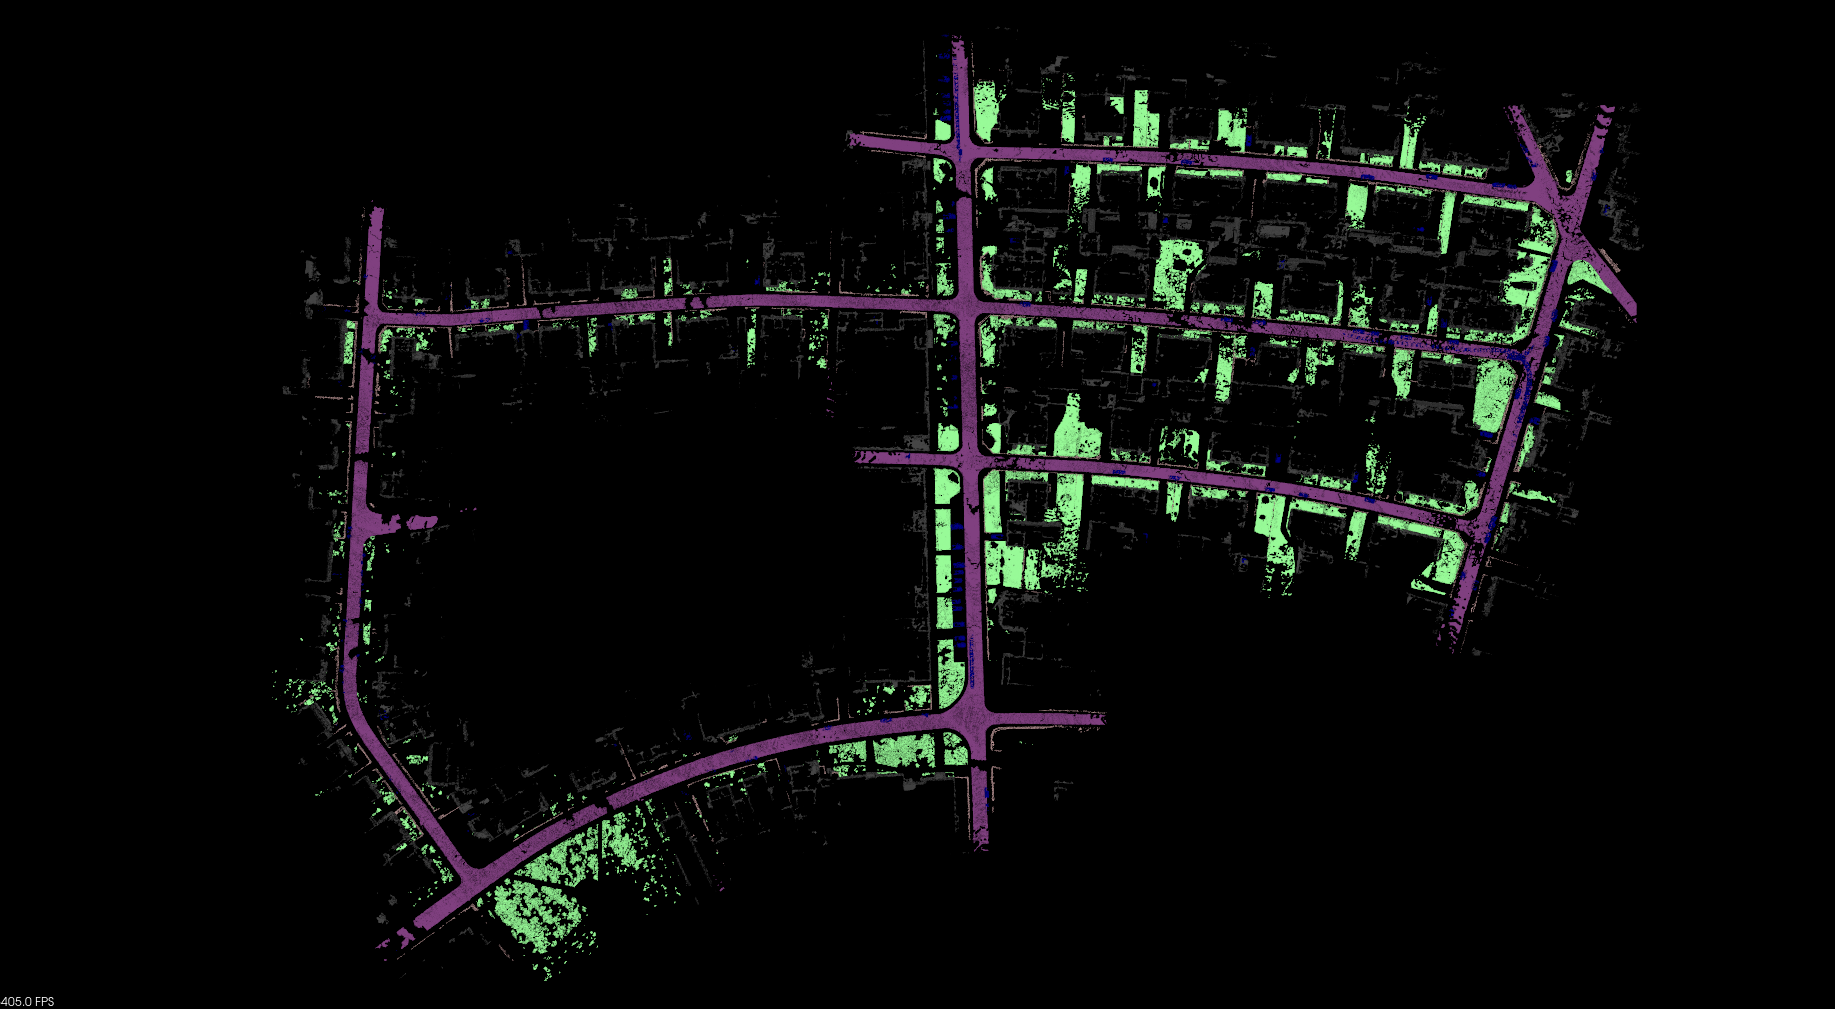
\includegraphics[width=75mm]{./picture/sequence05_map.png}
  \end{center}
  \caption{Sequence05}
  \label{fig:sequence05}
 \end{minipage}
 \begin{minipage}{0.5\hsize}
  \begin{center}
   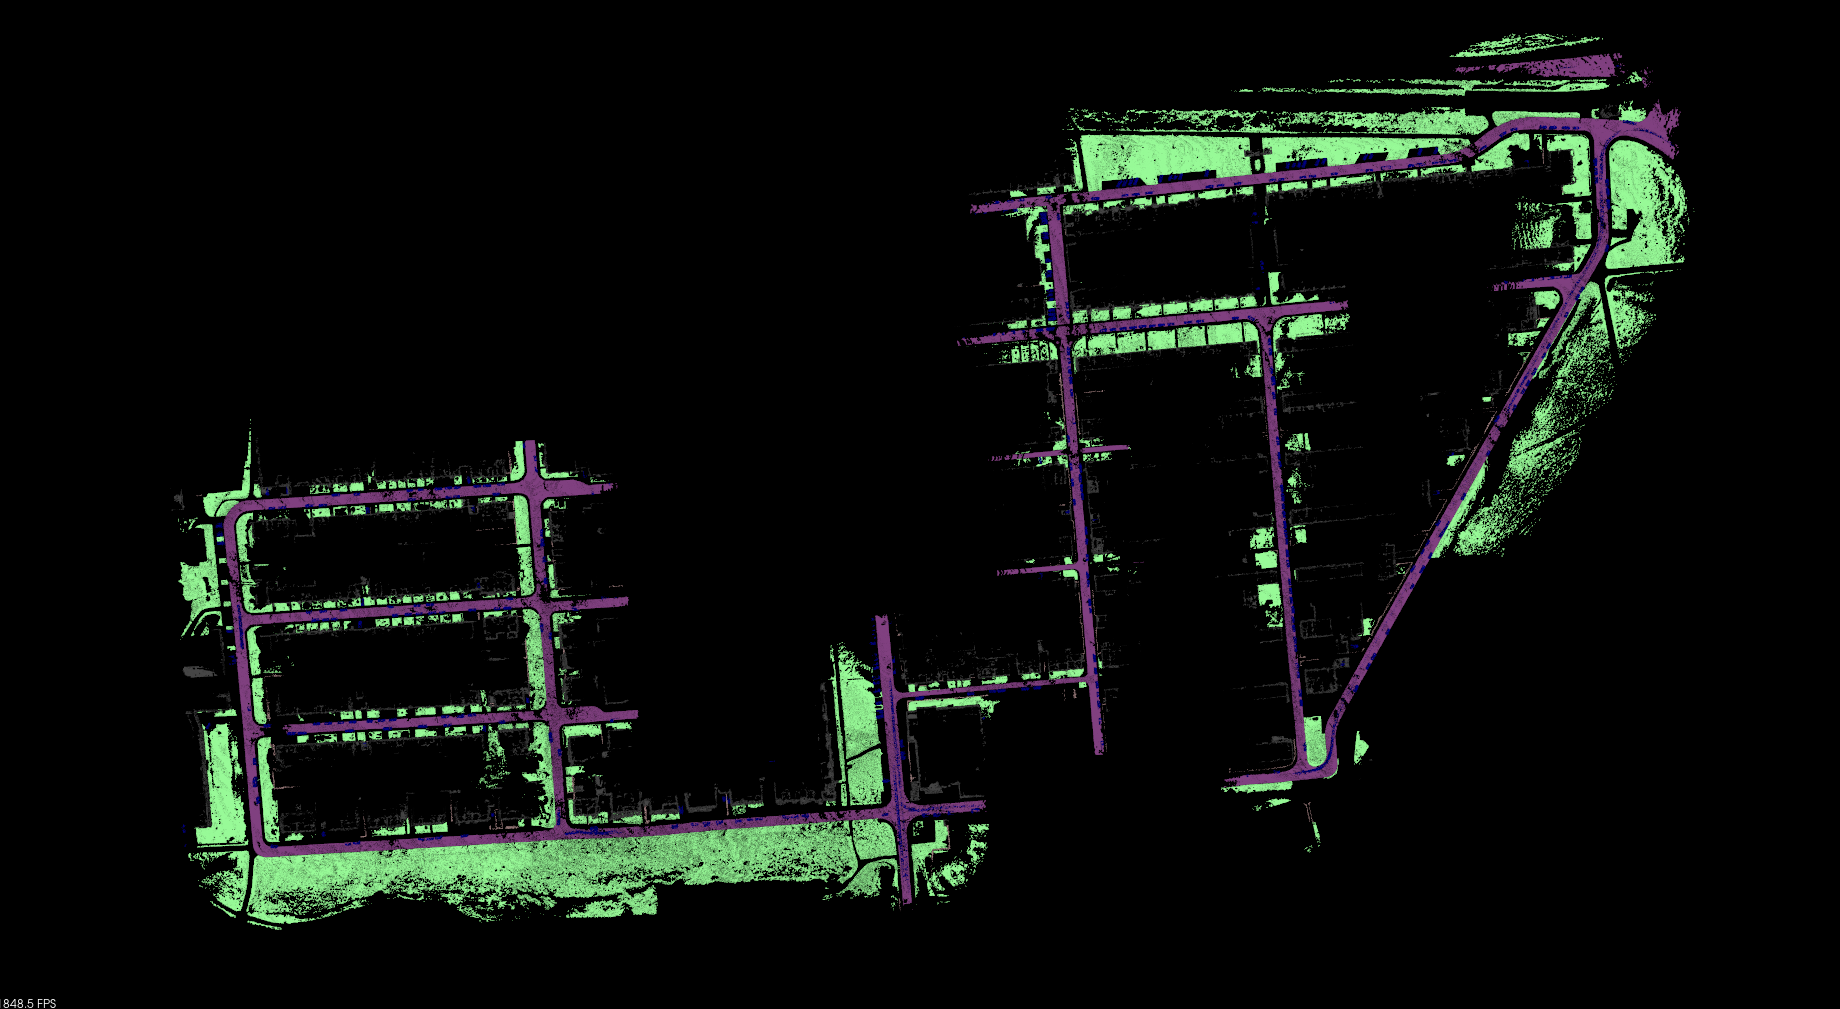
\includegraphics[width=75mm]{./picture/sequence08_map.png}
  \end{center}
  \caption{Sequence08}
  \label{fig:sequence08}
 \end{minipage}
\end{figure}

\begin{table}[htbp]
\begin{center}
\caption{Semantic KITTI dataset から得られるデータ}\label{tab:data_from_semantic_kitti}
  \begin{tabular}{l|l} \hline
    \multicolumn{1}{c|}{データ名} & \multicolumn{1}{c}{備考} \\ \hline
    点群データ & 車や建物などラベルが付与されている \\
    画像データ & 前方に搭載したRGBカメラとモノクロカメラから画像データが得られる \\
    Ground Truth & 精度評価, 及び誤差を含むオドメトリの生成に用いる\\
    固定位置関係 & LiDARとカメラ間の位置関係など時間変化のしない位置関係のデータ \\ \hline
  \end{tabular}
\end{center}
\end{table}

%% odometryの値が真値だからランダムに誤差与えました的なことを書く
%%尤度算出のパラメーターや分散の値を書く
\section{補足}\label{sec:env_appendix}
今回の実験においてモンテカルロ自己位置推定におけるハイパーパラメータを表\ref{tab:MCL_parameter}, 尤度算出におけるハイパーパラメータを表\ref{tab:likelihood_parameter}に示す. また, 表\ref{tab:likelihood_parameter}の値はAlg.\ref{alg:calc_likelihood}における関数semantic score()の出力値である.

\begin{table}[htbp]
\begin{center}
\caption{メッシュ地図での自己位置推定におけるハイパーパラメータ}
  \begin{tabular}{l|r|l} \hline
    \multicolumn{1}{c|}{パラメータ名} & \multicolumn{1}{c|}{値} & \multicolumn{1}{c}{役割} \\ \hline
    BiasXY & 0.030 & 正規分布に従うオドメトリのXY方向の誤差の分散 \\
    BiasZ & 0.020 & 正規分布に従うオドメトリのZ方向の誤差の分散 \\
    BiasRPY & 0.020 & 正規分布に従うオドメトリのRPY方向の誤差の分散 \\
    XDev & 0.300 & 正規分布に従って広がるパーティクルのX方向の分散 \\
    YDev & 0.300 & 正規分布に従って広がるパーティクルのY方向の分散 \\
    ZDev & 0.130 & 正規分布に従って広がるパーティクルのZ方向の分散 \\
    RollDev & 0.015 & 正規分布に従って広がるパーティクルのRoll方向の分散 \\
    PitchDev & 0.015 & 正規分布に従って広がるパーティクルのPitch方向の分散 \\
    YawDev & 0.015 & 正規分布に従って広がるパーティクルのYaw方向の分散 \\
    ImageDownWidth & 0.250 & カメラ画像のサイズ変更の比率, 処理軽減のため \\
    ImageDownHeight & 0.250 & カメラ画像のサイズ変更の比率, 処理軽減のため \\
    ParticleNumber & 100 & モンテカルロ自己位置推定におけるパーティクルの数 \\
    Averagenumber & 5 & \ref{sec:estimate_current_pose}節の処理にて上位何個のパーティクルの平均を取るか \\ \hline
  \end{tabular}
  \label{tab:MCL_parameter}
\end{center}
\end{table}

\begin{table}[htbp]
\begin{center}
\caption{尤度算出におけるハイパーパラメータ}
  \begin{tabular}{l c l} \hline
    クラス & 値 & 補足\\ \hline
    Road & 0.7 & \\
    Sidewalk & 1.5 & \\
    Car & 4.0 & \\
    Building & 0.7 & \\
    Terrain & 2.0 & 芝生を指す\\
    Other Class & 1.0 & \\ \hline
  \end{tabular}
  \label{tab:likelihood_parameter}
\end{center}
\end{table}


%% 実験結果&考察
\chapter{実験結果}

%% 市街地でのシークエンスでの走行結果を書く
\section{実験結果}\label{sec:result}

\subsection{自己位置推定の精度}\label{sec:verify_localization}

\subsubsection{XYZ座標推定の精度}
メッシュ地図及び点群地図における自己位置推定において, 自己位置推定によって推定された位置とground truthとの間にどれほどの差があったかを割合で図\ref{fig:mesh_sequence00_XYZ}から図\ref{fig:point_sequence08_XYZ}にかけて示す. また, 実験においてGround truthの移動量からガウス分布に従う誤差を加えたオドメトリを用いて事前分布の更新を行った. このとき用いたオドメトリ, 「biased odometry」の位置とGround truthの位置との間にどれほどの差があったかも併せて図に示す.
\par 先行研究\cite{semantic_point_localization}については論文内では精度のいい自己位置推定の結果が示されていたが今回の実験においてはいずれのシークエンスでも自己位置推定が完全に破綻しており有効な結果は得られなかった. その一方で提案手法はいずれのシークエンスでも自己位置推定が破綻することなく安定した動作が見られた. しかしsequence05を除き, いずれのシークエンスでも1.5m以上2.0m以下の誤差が最頻値であったことから提案手法は今回の実験環境においては数cm単位での高い自己位置推定の精度を保証するものではない事が判明した. また, 時速30km以上での走行を行っているときは先行研究での手法と提案手法の両方で正確な自己位置推定ができなくなった. sequence05において自己位置推定がどの手法でも破綻したのはこのためであり, この原因については\ref{sec:considerarion}節で詳しく述べる.

\subsubsection{RPY方向推定の精度}
メッシュ地図及び点群地図における自己位置推定において, 自己位置推定によって推定された角度とground truthとの間にどれほどの差があったかを割合で図\ref{fig:mesh_sequence00_RPY}から図\ref{fig:point_sequence08_RPY}にかけて示す. \par 既存手法による角度推定ではsequence08等においてground truthと大きく異る値になることが頻繁に起こっていたが, 提案手法による角度推定においてはいずれのシークエンスでも誤差が概ね10度以下に収まるといった良好な結果が得られた.

\begin{figure}[htbp]
 \begin{minipage}{1.0\hsize}
  \begin{center}
   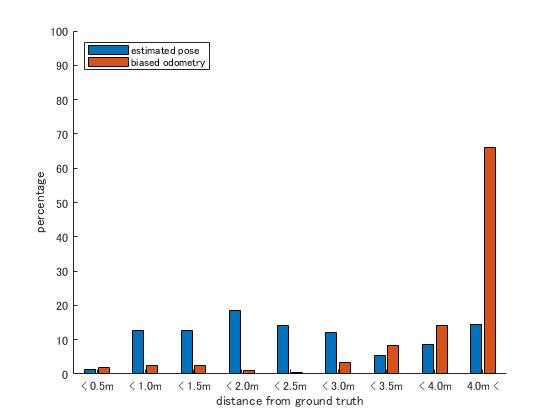
\includegraphics[width=110mm]{./picture/mesh_s0_xyz.jpg}
  \end{center}
  \caption{Sequence00における提案手法での自己位置推定精度}
  \label{fig:mesh_sequence00_XYZ}
 \end{minipage}
\end{figure}

\begin{figure}[htbp]
 \begin{minipage}{1.0\hsize}
  \begin{center}
   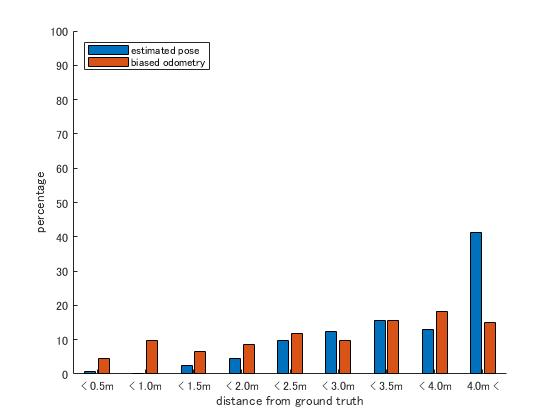
\includegraphics[width=110mm]{./picture/point_s0_xyz.jpg}
  \end{center}
  \caption{Sequence00における比較手法での自己位置推定精度}
  \label{fig:point_sequence00_XYZ}
 \end{minipage}
\end{figure}
 
\begin{figure}[htbp]
  \begin{minipage}{1.0\hsize}
  \begin{center}
   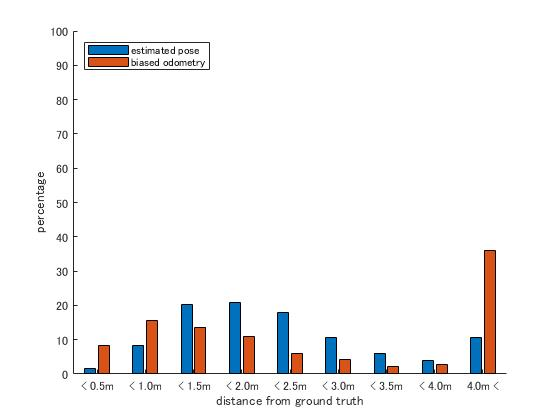
\includegraphics[width=110mm]{./picture/mesh_s2_xyz.jpg}
  \end{center}
  \caption{Sequence02における提案手法での自己位置推定精度}
  \label{fig:mesh_sequence02_XYZ}
 \end{minipage}
\end{figure}

\begin{figure}[htbp]
 \begin{minipage}{1.0\hsize}
  \begin{center}
   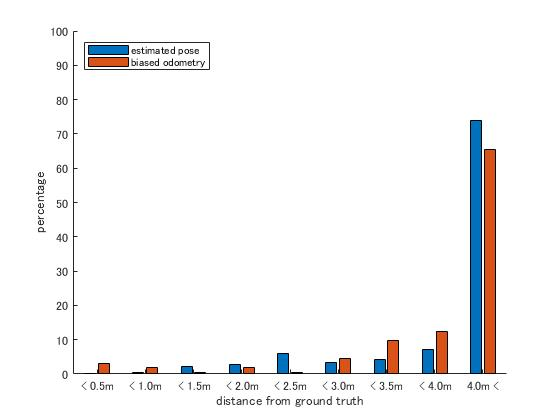
\includegraphics[width=110mm]{./picture/point_s2_xyz.jpg}
  \end{center}
  \caption{Sequence02における比較手法での自己位置推定精度}
  \label{fig:point_sequence02_XYZ}
 \end{minipage}
\end{figure}

\begin{figure}[htbp]
  \begin{minipage}{1.0\hsize}
  \begin{center}
   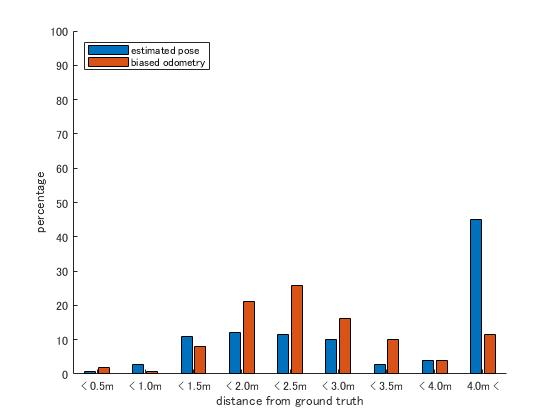
\includegraphics[width=110mm]{./picture/mesh_s5_xyz.jpg}
  \end{center}
  \caption{Sequence05における提案手法での自己位置推定精度}
  \label{fig:mesh_sequence05_XYZ}
 \end{minipage}
\end{figure}

\begin{figure}[htbp]
 \begin{minipage}{1.0\hsize}
  \begin{center}
   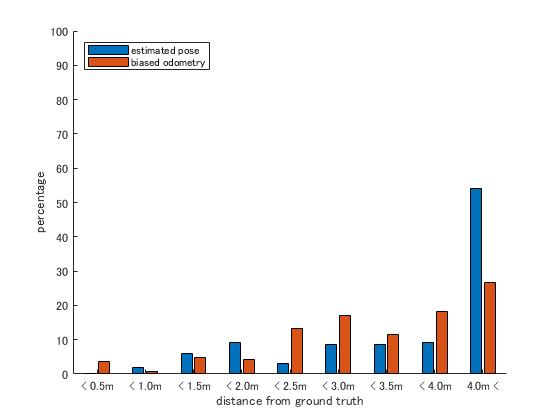
\includegraphics[width=110mm]{./picture/point_s5_xyz.jpg}
  \end{center}
  \caption{Sequence05における比較手法での自己位置推定精度}
  \label{fig:point_sequence05_XYZ}
 \end{minipage}
\end{figure}

\begin{figure}[htbp]
  \begin{minipage}{1.0\hsize}
  \begin{center}
   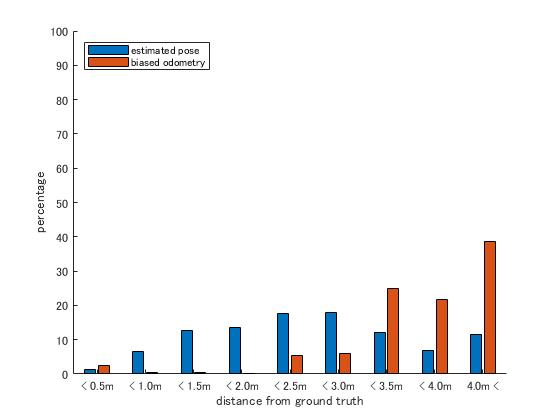
\includegraphics[width=110mm]{./picture/mesh_s8_xyz.jpg}
  \end{center}
  \caption{Sequence08における提案手法での自己位置推定精度}
  \label{fig:mesh_sequence08_XYZ}
 \end{minipage}
\end{figure}

\begin{figure}[htbp]
 \begin{minipage}{1.0\hsize}
  \begin{center}
   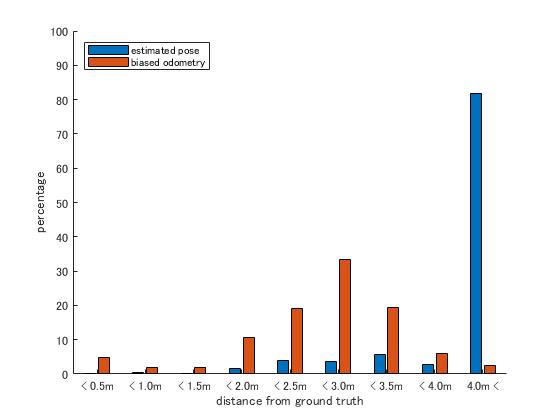
\includegraphics[width=110mm]{./picture/point_s8_xyz.jpg}
  \end{center}
  \caption{Sequence08における比較手法での自己位置推定精度}
  \label{fig:point_sequence08_XYZ}
 \end{minipage}
\end{figure}


\begin{figure}[htbp]
 \begin{minipage}{1.0\hsize}
  \begin{center}
   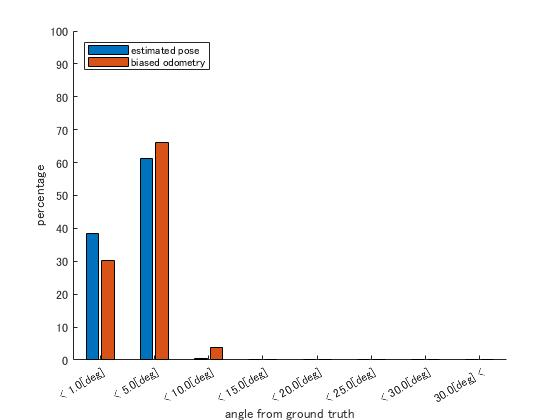
\includegraphics[width=110mm]{./picture/mesh_s0_rpy.jpg}
  \end{center}
  \caption{Sequence00における提案手法での角度推定精度}
  \label{fig:mesh_sequence00_RPY}
 \end{minipage}
\end{figure}

\begin{figure}[htbp]
 \begin{minipage}{1.0\hsize}
  \begin{center}
   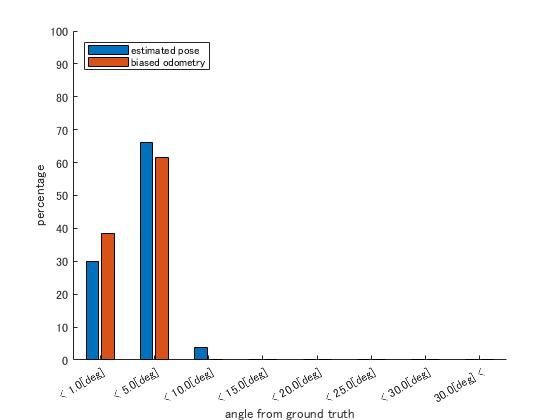
\includegraphics[width=110mm]{./picture/point_s0_rpy.jpg}
  \end{center}
  \caption{Sequence00における比較手法での角度推定精度}
  \label{fig:point_sequence00_RPY}
 \end{minipage}
\end{figure}
 
\begin{figure}[htbp]
  \begin{minipage}{1.0\hsize}
  \begin{center}
   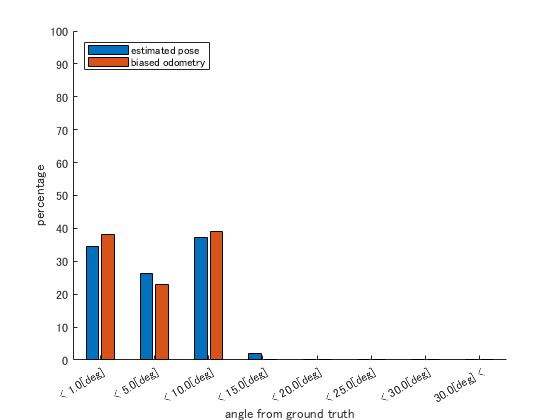
\includegraphics[width=110mm]{./picture/mesh_s2_rpy.jpg}
  \end{center}
  \caption{Sequence02における提案手法での角度推定精度}
  \label{fig:mesh_sequence02_RPY}
 \end{minipage}
\end{figure}

\begin{figure}[htbp]
 \begin{minipage}{1.0\hsize}
  \begin{center}
   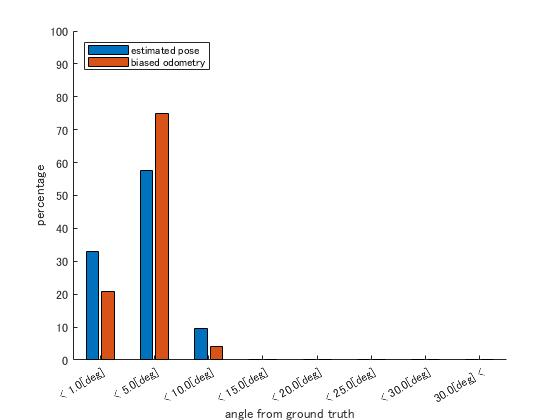
\includegraphics[width=110mm]{./picture/point_s2_rpy.jpg}
  \end{center}
  \caption{Sequence02における比較手法での角度推定精度}
  \label{fig:point_sequence02_RPY}
 \end{minipage}
\end{figure}

\begin{figure}[htbp]
  \begin{minipage}{1.0\hsize}
  \begin{center}
   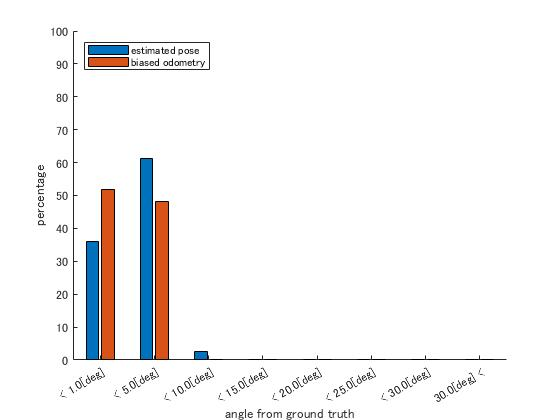
\includegraphics[width=110mm]{./picture/mesh_s5_rpy.jpg}
  \end{center}
  \caption{Sequence05における提案手法での角度推定精度}
  \label{fig:mesh_sequence05_RPY}
 \end{minipage}
\end{figure}

\begin{figure}[htbp]
 \begin{minipage}{1.0\hsize}
  \begin{center}
   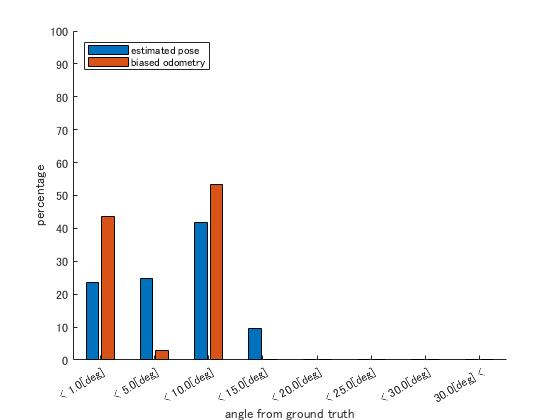
\includegraphics[width=110mm]{./picture/point_s5_rpy.jpg}
  \end{center}
  \caption{Sequence05における比較手法での角度推定精度}
  \label{fig:point_sequence05_RPY}
 \end{minipage}
\end{figure}

\begin{figure}[htbp]
  \begin{minipage}{1.0\hsize}
  \begin{center}
   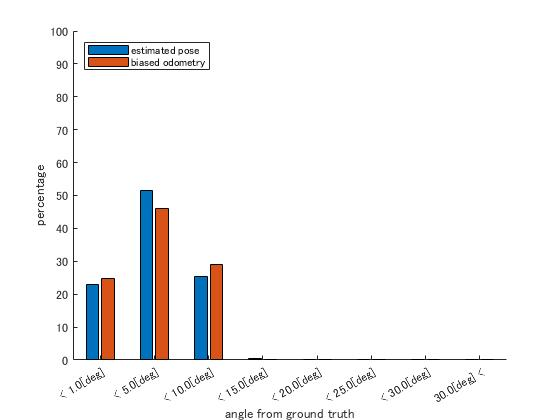
\includegraphics[width=110mm]{./picture/mesh_s8_rpy.jpg}
  \end{center}
  \caption{Sequence08における提案手法での角度推定精度}
  \label{fig:mesh_sequence08_RPY}
 \end{minipage}
\end{figure}

\begin{figure}[htbp]
 \begin{minipage}{1.0\hsize}
  \begin{center}
   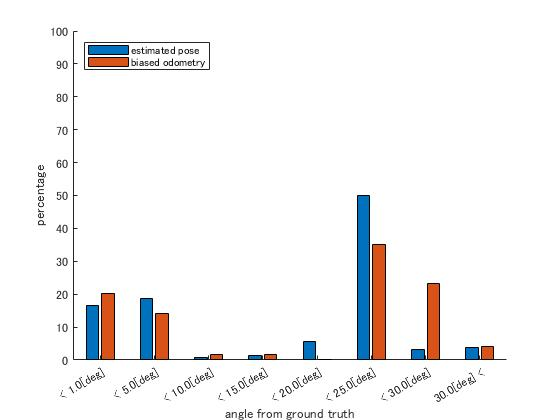
\includegraphics[width=110mm]{./picture/point_s8_rpy.jpg}
  \end{center}
  \caption{Sequence08における比較手法での角度推定精度}
  \label{fig:point_sequence08_RPY}
 \end{minipage}
\end{figure}


\subsection{尤度算出の評価}\label{sec:verify_likelihood}

%\subsubsection{水平変化に対する評価}

%\subsubsection{角度変化に対する評価}

\subsubsection{先行研究との評価}
提案手法における尤度算出の有効性を示すために, 時刻$t$における真の位置$x_{t}^{*}$からみたメッシュ地図と点群地図の風景をそれぞれ画像化してセグメンテーションされたカメラ画像$z_{t}$と比較, セマンティックなクラスが一致したピクセルの数を計測した. Sequence00の中から異なる13の位置を記録して先程述べた手法により比較を行った. この時の13の位置は図\ref{fig:sequence00_place}のとおりである. 全ピクセルの内何\%が一致していると判断されたかの結果を表\ref{tab:cmp_calc_likelihood}に示す. なお, 実験にあたり表\ref{tab:MCL_parameter}のimagedownwidthとimagedownheightを1.0に調整した. また, 各位置におけるカメラ画像, セグメンテーションされた画像, メッシュ地図, 点群地図, メッシュ地図と点群地図においてクラスが一致していると判断されたピクセルのみを抽出した画像を図\ref{fig:place1}から図\ref{fig:place13}にかけて示す. 

\begin{table}[htbp]
\begin{center}
\caption{メッシュ地図と点群地図での尤度算出の比較}
  \begin{tabular}{|c|r|r|} \hline
    地点 & メッシュ地図(\%) & 点群地図(\%)\\ \hline
    1 & 22.3 & 4.0 \\ \hline
    2 & 11.1 & 2.4 \\ \hline
    3 & 25.1 & 8.1 \\ \hline
    4 & 41.2 & 5.8 \\ \hline
    5 & 27.4 & 3.9 \\ \hline
    6 & 26.6 & 2.8 \\ \hline
    7 & 25.8 & 5.0 \\ \hline
    8 & 36.5 & 5.1 \\ \hline
    9 & 30.8 & 5.8 \\ \hline
    10 & 13.2 & 1.5 \\ \hline
    11 & 14.0 & 1.8 \\ \hline
    12 & 17.3 & 2.3 \\ \hline
    13 & 30.3 & 4.5 \\ \hline

  \end{tabular}
  \label{tab:cmp_calc_likelihood}
\end{center}
\end{table}

\begin{figure}[htpb]
\begin{minipage}[b]{1.0\hsize}
\begin{center}
    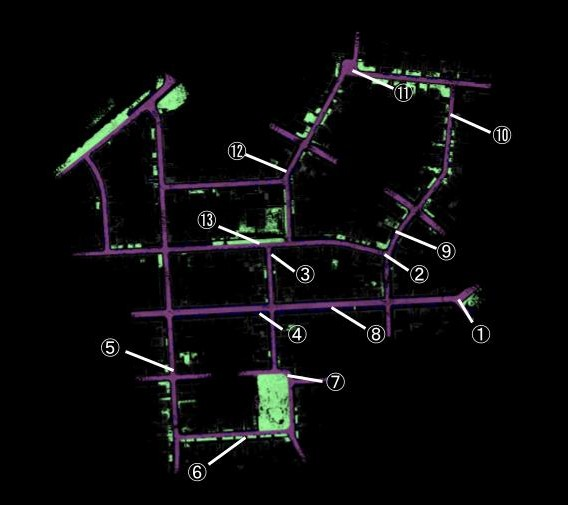
\includegraphics[width=120mm]{./picture/sequence00_pointmap.jpg}
\end{center}
\caption{尤度算出の検証において選定された地点}
\label{fig:sequence00_place}
\end{minipage}
\end{figure}

\begin{figure}[htbp]
 \begin{minipage}[b]{0.50\hsize}
 \begin{center}
  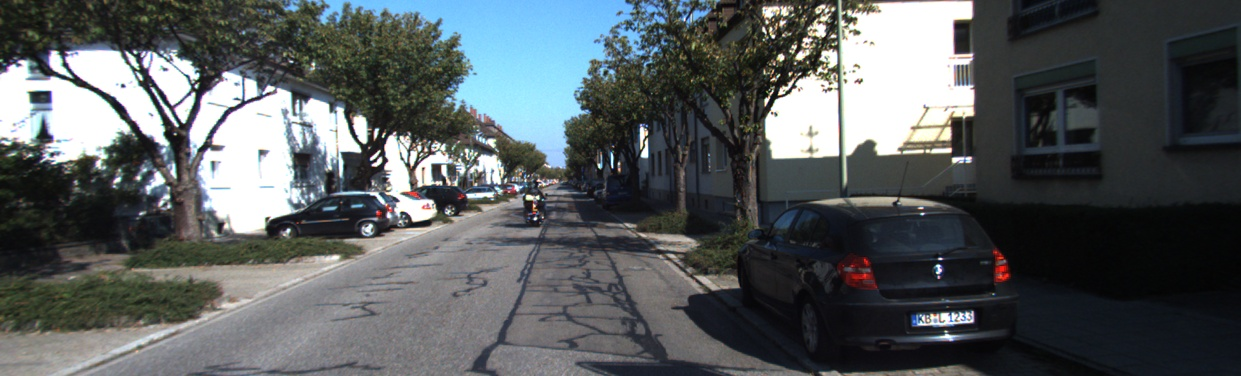
\includegraphics[keepaspectratio, scale=0.18]{./picture/bgrimage/bgrimage0.jpg}
  \subcaption{カメラ画像}
  \end{center}
 \end{minipage}
 \begin{minipage}[b]{0.5\hsize}
 \begin{center}
  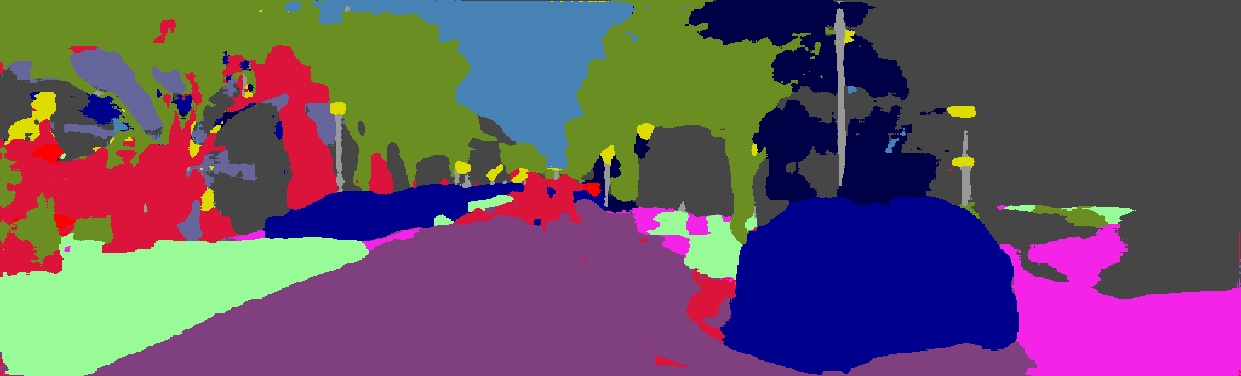
\includegraphics[keepaspectratio, scale=0.18]{./picture/segimage/image0.jpg}
  \subcaption{セグメンテーションされた画像}
  \end{center}
 \end{minipage} \\
 \begin{minipage}[b]{0.50\hsize}
 \begin{center}
  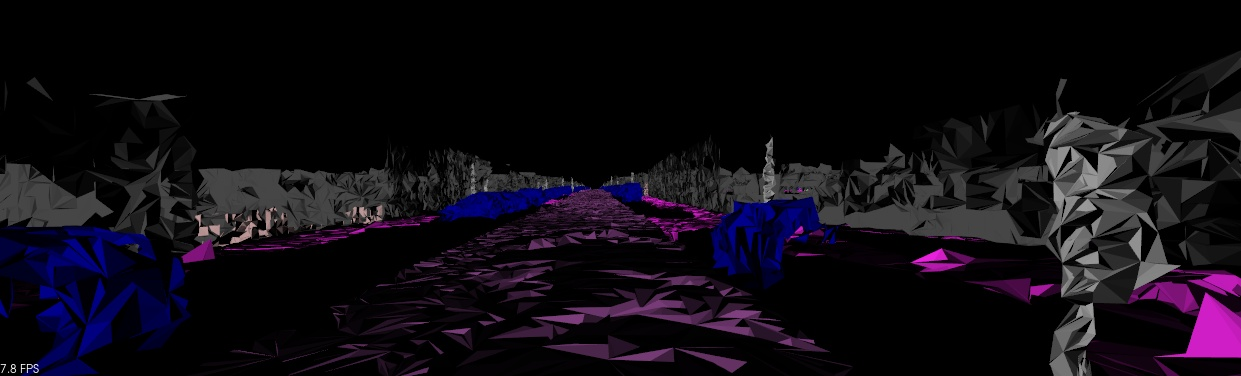
\includegraphics[keepaspectratio, scale=0.18]{./picture/mesh_map_image/image0.jpg}
  \subcaption{メッシュ地図}
  \end{center}
 \end{minipage}
 \begin{minipage}[b]{0.50\hsize}
 \begin{center}
  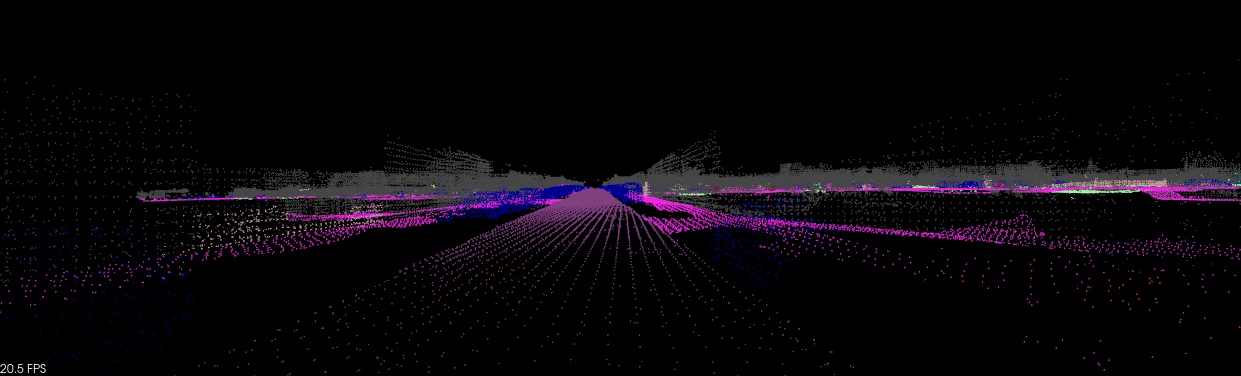
\includegraphics[keepaspectratio, scale=0.18]{./picture/point_map_image/image0.jpg}
  \subcaption{点群地図}
  \end{center}
 \end{minipage} \\
  \begin{minipage}[b]{0.50\hsize}
 \begin{center}
  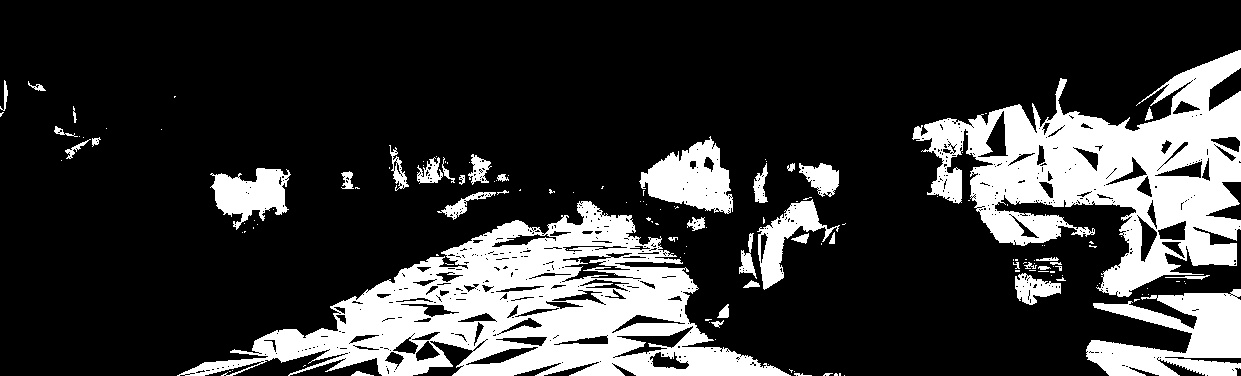
\includegraphics[keepaspectratio, scale=0.18]{./picture/valued_mesh_map_image/image0.jpg}
  \subcaption{メッシュ地図にてクラスが一致したピクセル}
  \end{center}
 \end{minipage}
 \begin{minipage}[b]{0.50\hsize}
 \begin{center}
  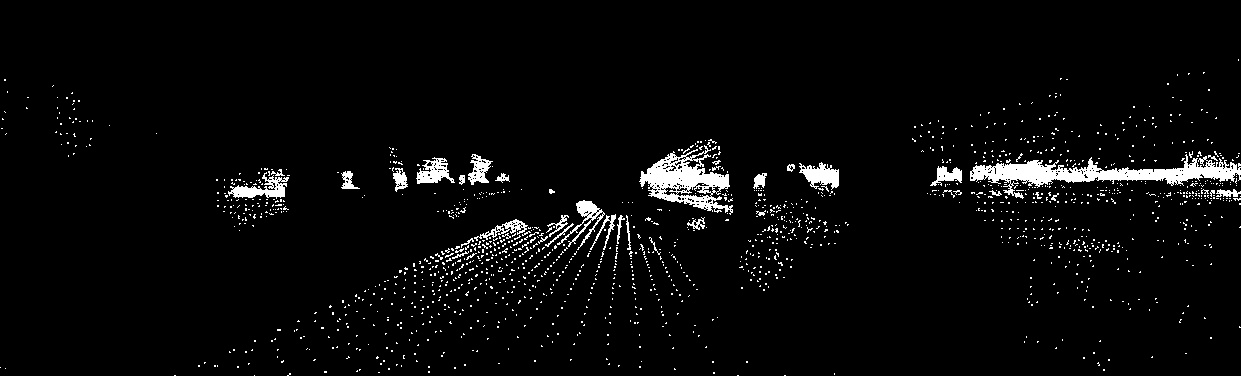
\includegraphics[keepaspectratio, scale=0.18]{./picture/valued_point_map_image/image0.jpg}
  \subcaption{点群地図にてクラスが一致したピクセル}
  \end{center}
 \end{minipage}
 \caption{位置1でのカメラ画像, セグメンテーションされた画像, メッシュ地図, 点群地図}\label{fig:place1}
\end{figure}

\par

\begin{figure}[htbp]
 \begin{minipage}[b]{0.50\hsize}
 \begin{center}
  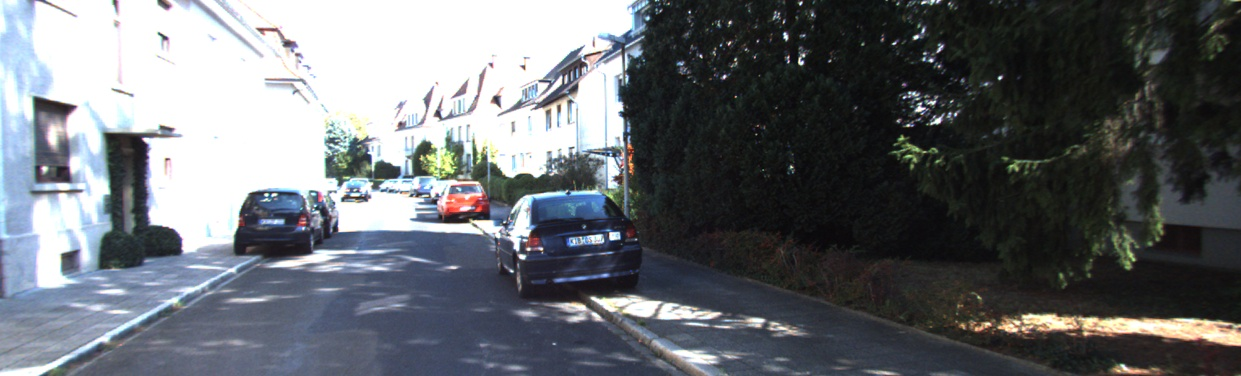
\includegraphics[keepaspectratio, scale=0.18]{./picture/bgrimage/bgrimage1.jpg}
  \subcaption{カメラ画像}
  \end{center}
 \end{minipage}
 \begin{minipage}[b]{0.5\hsize}
 \begin{center}
  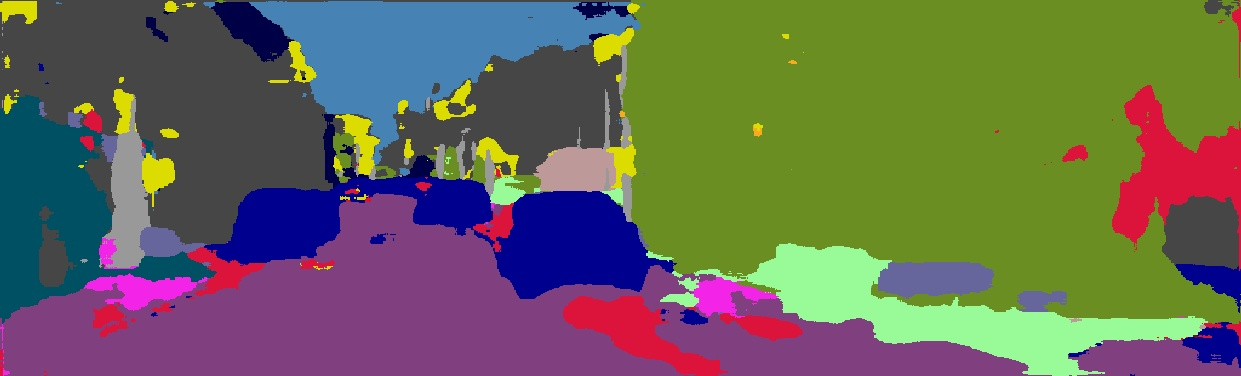
\includegraphics[keepaspectratio, scale=0.18]{./picture/segimage/image1.jpg}
  \subcaption{セグメンテーションされた画像}
  \end{center}
 \end{minipage} \\
 \begin{minipage}[b]{0.50\hsize}
 \begin{center}
  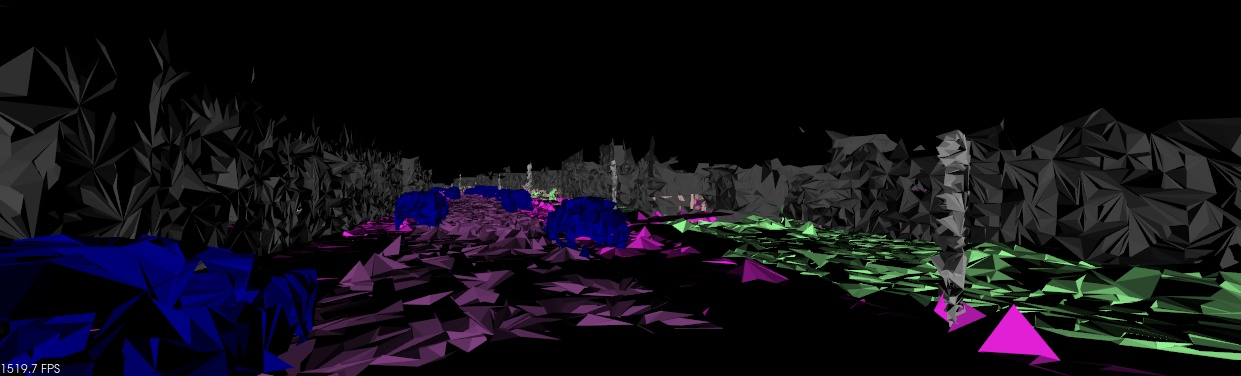
\includegraphics[keepaspectratio, scale=0.18]{./picture/mesh_map_image/image1.jpg}
  \subcaption{メッシュ地図}
  \end{center}
 \end{minipage}
 \begin{minipage}[b]{0.50\hsize}
 \begin{center}
  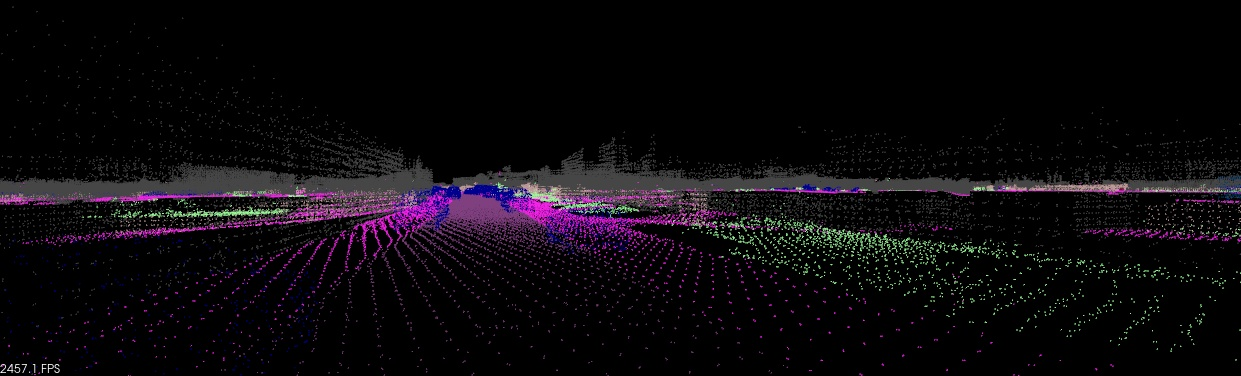
\includegraphics[keepaspectratio, scale=0.18]{./picture/point_map_image/image1.jpg}
  \subcaption{点群地図}
  \end{center}
 \end{minipage} \\
   \begin{minipage}[b]{0.50\hsize}
 \begin{center}
  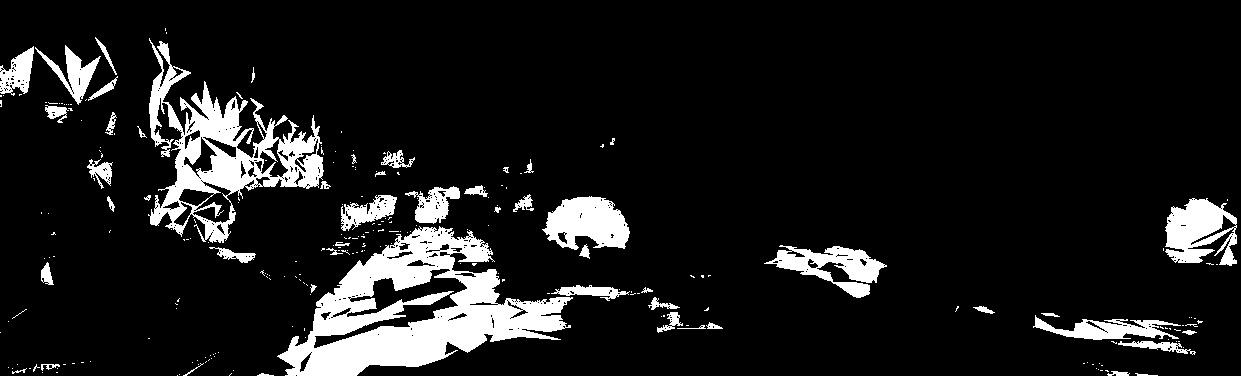
\includegraphics[keepaspectratio, scale=0.18]{./picture/valued_mesh_map_image/image1.jpg}
  \subcaption{メッシュ地図にてクラスが一致したピクセル}
  \end{center}
 \end{minipage}
 \begin{minipage}[b]{0.50\hsize}
 \begin{center}
  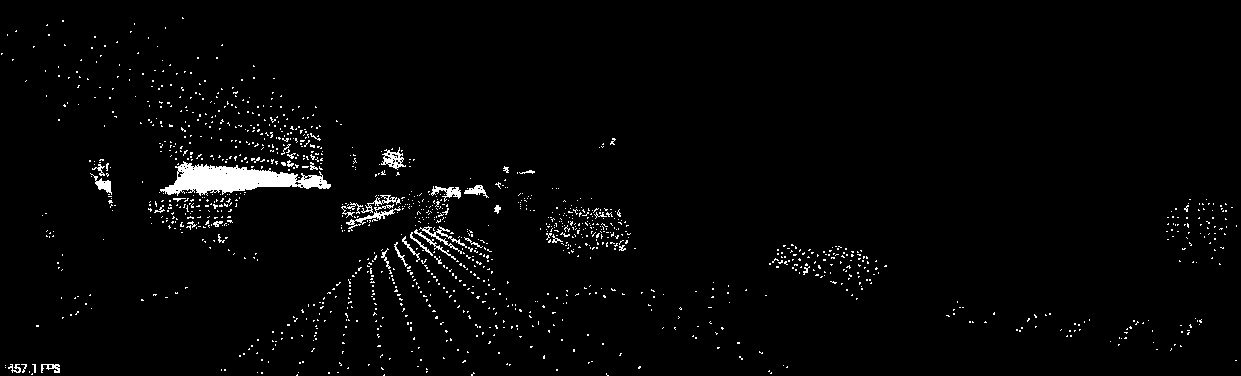
\includegraphics[keepaspectratio, scale=0.18]{./picture/valued_point_map_image/image1.jpg}
  \subcaption{点群地図にてクラスが一致したピクセル}
  \end{center}
 \end{minipage}
 \caption{位置2でのカメラ画像, セグメンテーションされた画像, メッシュ地図, 点群地図}\label{fig:place2}
\end{figure}

\begin{figure}[htbp]
 \begin{minipage}[b]{0.50\hsize}
 \begin{center}
  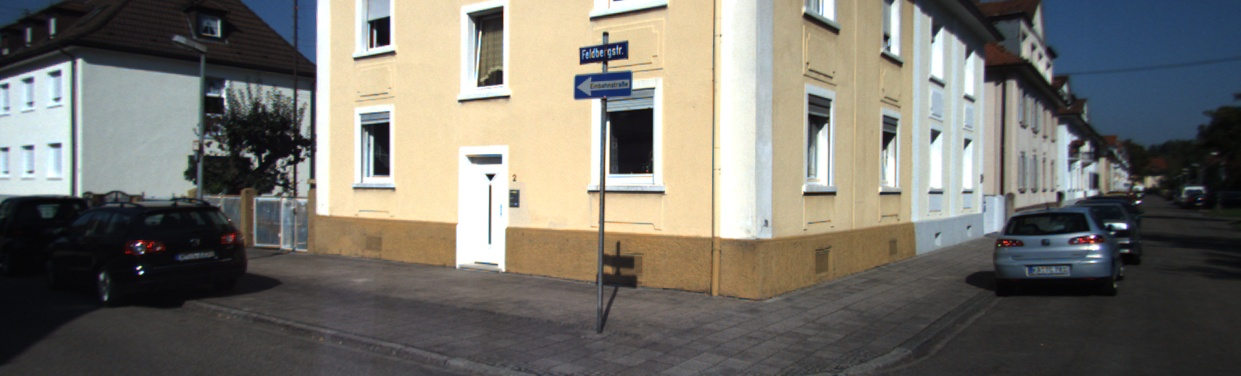
\includegraphics[keepaspectratio, scale=0.18]{./picture/bgrimage/bgrimage2.jpg}
  \subcaption{カメラ画像}
  \end{center}
 \end{minipage}
 \begin{minipage}[b]{0.5\hsize}
 \begin{center}
  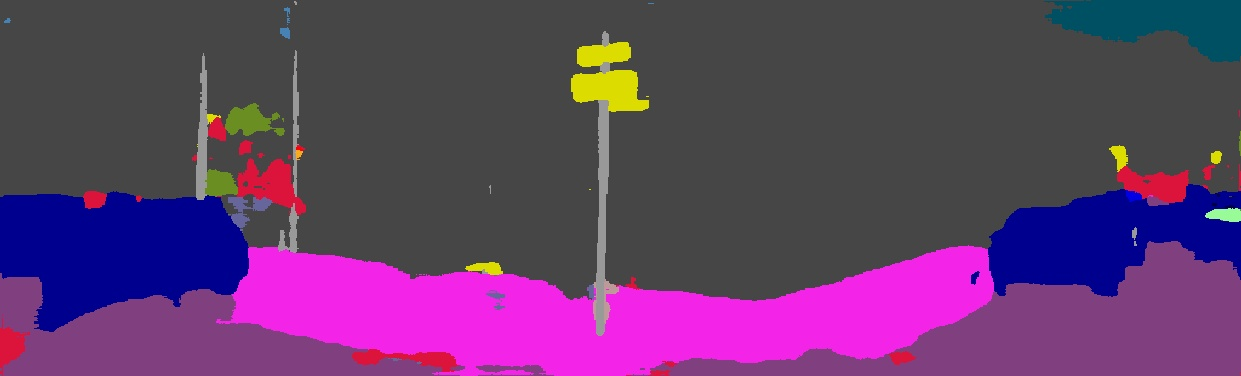
\includegraphics[keepaspectratio, scale=0.18]{./picture/segimage/image2.jpg}
  \subcaption{セグメンテーションされた画像}
  \end{center}
 \end{minipage} \\
 \begin{minipage}[b]{0.50\hsize}
 \begin{center}
  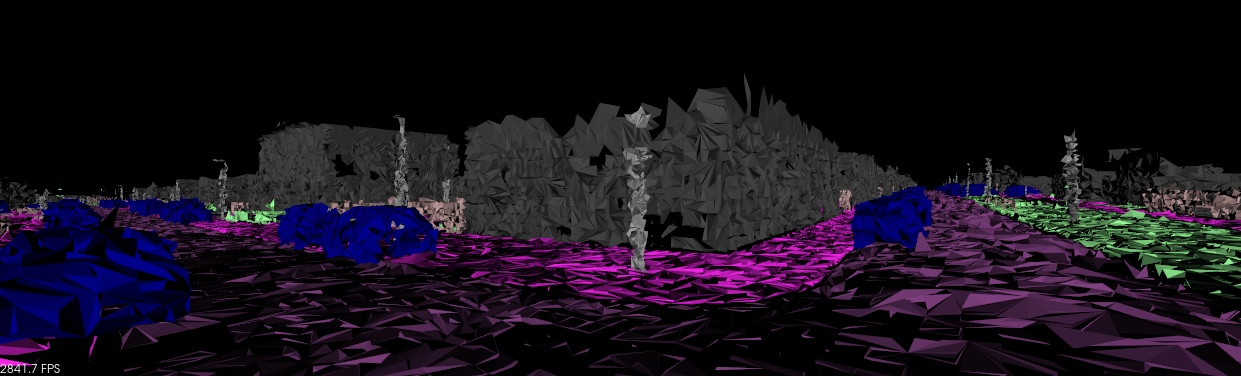
\includegraphics[keepaspectratio, scale=0.18]{./picture/mesh_map_image/image2.jpg}
  \subcaption{メッシュ地図}
  \end{center}
 \end{minipage}
 \begin{minipage}[b]{0.50\hsize}
 \begin{center}
  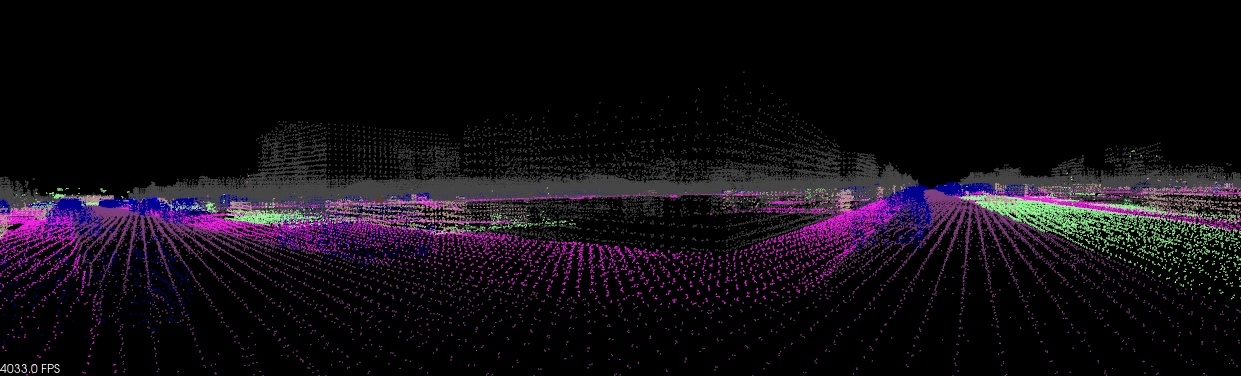
\includegraphics[keepaspectratio, scale=0.18]{./picture/point_map_image/image2.jpg}
  \subcaption{点群地図}
  \end{center}
 \end{minipage} \\
   \begin{minipage}[b]{0.50\hsize}
 \begin{center}
  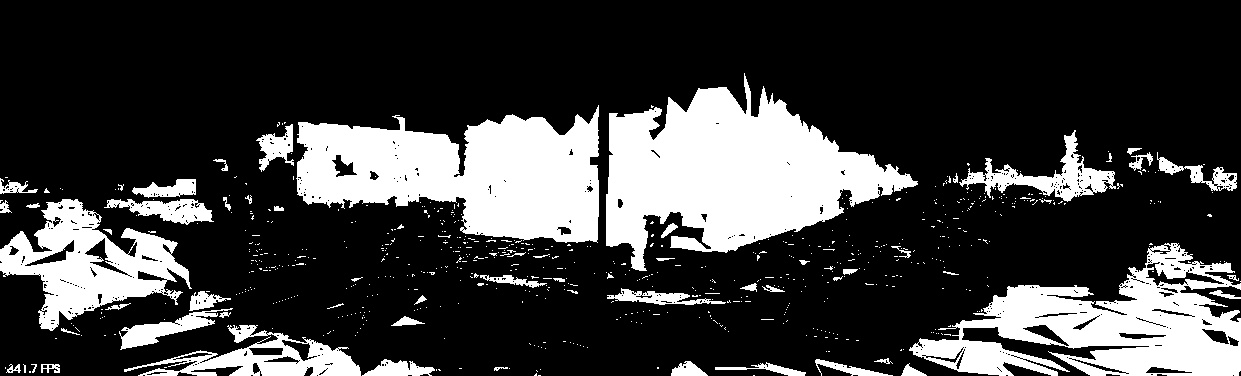
\includegraphics[keepaspectratio, scale=0.18]{./picture/valued_mesh_map_image/image2.jpg}
  \subcaption{メッシュ地図にてクラスが一致したピクセル}
  \end{center}
 \end{minipage}
 \begin{minipage}[b]{0.50\hsize}
 \begin{center}
  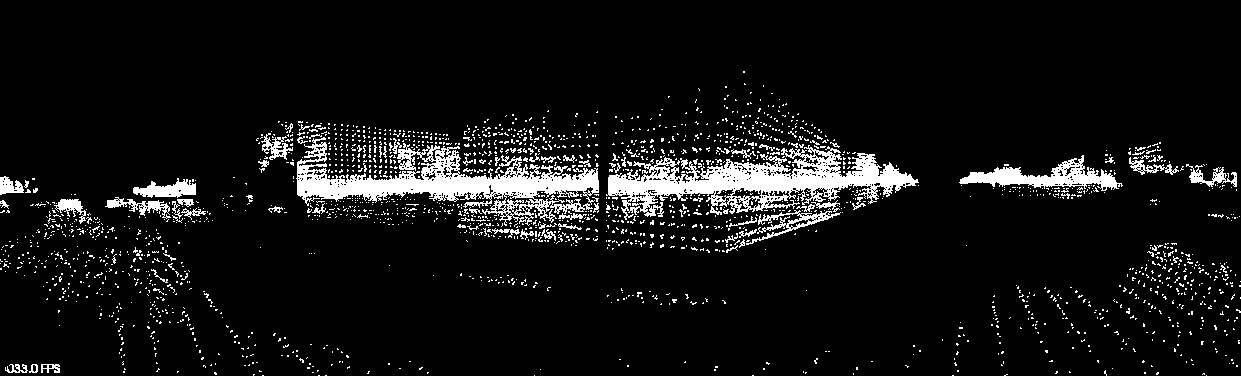
\includegraphics[keepaspectratio, scale=0.18]{./picture/valued_point_map_image/image2.jpg}
  \subcaption{点群地図にてクラスが一致したピクセル}
  \end{center}
 \end{minipage}
 \caption{位置3でのカメラ画像, セグメンテーションされた画像, メッシュ地図, 点群地図}\label{fig:place3}
\end{figure}


\begin{figure}[htbp]
 \begin{minipage}[b]{0.50\hsize}
 \begin{center}
  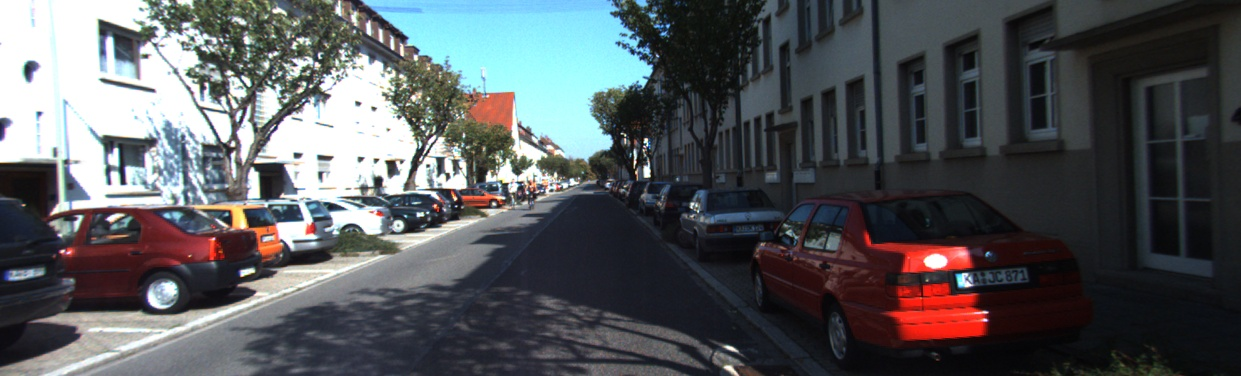
\includegraphics[keepaspectratio, scale=0.18]{./picture/bgrimage/bgrimage3.jpg}
  \subcaption{カメラ画像}
  \end{center}
 \end{minipage}
 \begin{minipage}[b]{0.5\hsize}
 \begin{center}
  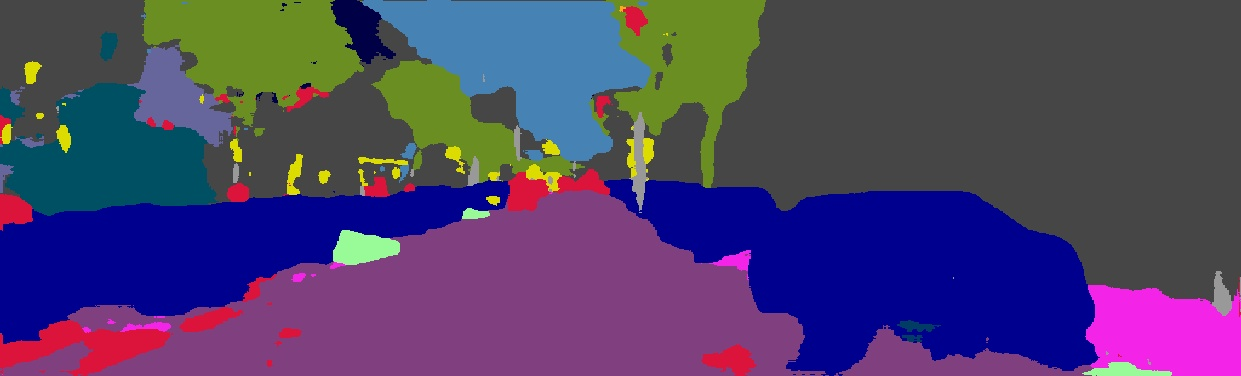
\includegraphics[keepaspectratio, scale=0.18]{./picture/segimage/image3.jpg}
  \subcaption{セグメンテーションされた画像}
  \end{center}
 \end{minipage} \\
 \begin{minipage}[b]{0.50\hsize}
 \begin{center}
  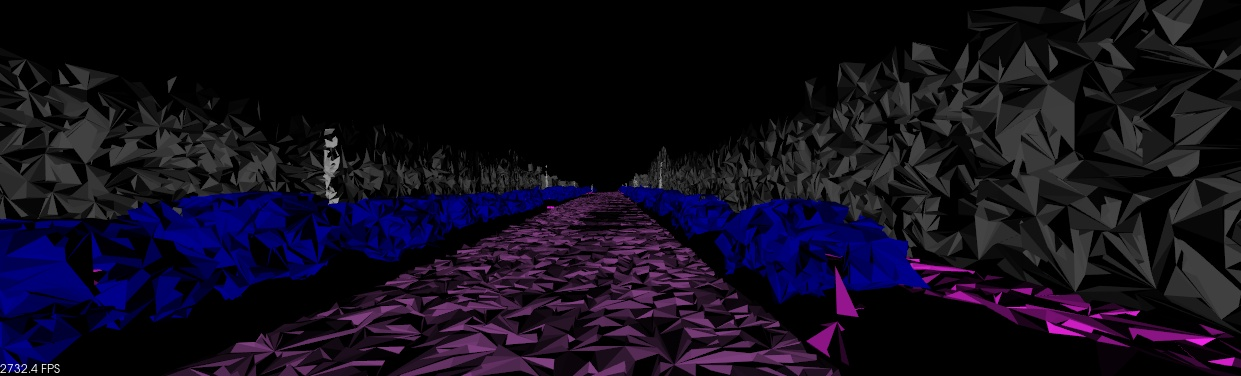
\includegraphics[keepaspectratio, scale=0.18]{./picture/mesh_map_image/image3.jpg}
  \subcaption{メッシュ地図}
  \end{center}
 \end{minipage}
 \begin{minipage}[b]{0.50\hsize}
 \begin{center}
  \includegraphics[keepaspectratio, scale=0.18]{./picture/point_map_image/image3.jpg}
  \subcaption{点群地図}
  \end{center}
 \end{minipage}\\
  \begin{minipage}[b]{0.50\hsize}
 \begin{center}
  \includegraphics[keepaspectratio, scale=0.18]{./picture/valued_mesh_map_image/image3.jpg}
  \subcaption{メッシュ地図にてクラスが一致したピクセル}
  \end{center}
 \end{minipage}
 \begin{minipage}[b]{0.50\hsize}
 \begin{center}
  \includegraphics[keepaspectratio, scale=0.18]{./picture/valued_point_map_image/image3.jpg}
  \subcaption{点群地図にてクラスが一致したピクセル}
  \end{center}
 \end{minipage}
 \caption{位置4でのカメラ画像, セグメンテーションされた画像, メッシュ地図, 点群地図}\label{fig:place4}
\end{figure}

\begin{figure}[htbp]
 \begin{minipage}[b]{0.50\hsize}
 \begin{center}
  \includegraphics[keepaspectratio, scale=0.18]{./picture/bgrimage/bgrimage4.jpg}
  \subcaption{カメラ画像}
  \end{center}
 \end{minipage}
 \begin{minipage}[b]{0.5\hsize}
 \begin{center}
  \includegraphics[keepaspectratio, scale=0.18]{./picture/segimage/image4.jpg}
  \subcaption{セグメンテーションされた画像}
  \end{center}
 \end{minipage} \\
 \begin{minipage}[b]{0.50\hsize}
 \begin{center}
  \includegraphics[keepaspectratio, scale=0.18]{./picture/mesh_map_image/image4.jpg}
  \subcaption{メッシュ地図}
  \end{center}
 \end{minipage}
 \begin{minipage}[b]{0.50\hsize}
 \begin{center}
  \includegraphics[keepaspectratio, scale=0.18]{./picture/point_map_image/image4.jpg}
  \subcaption{点群地図}
  \end{center}
 \end{minipage}\\
  \begin{minipage}[b]{0.50\hsize}
 \begin{center}
  \includegraphics[keepaspectratio, scale=0.18]{./picture/valued_mesh_map_image/image4.jpg}
  \subcaption{メッシュ地図にてクラスが一致したピクセル}
  \end{center}
 \end{minipage}
 \begin{minipage}[b]{0.50\hsize}
 \begin{center}
  \includegraphics[keepaspectratio, scale=0.18]{./picture/valued_point_map_image/image4.jpg}
  \subcaption{点群地図にてクラスが一致したピクセル}
  \end{center}
 \end{minipage}
 \caption{位置5でのカメラ画像, セグメンテーションされた画像, メッシュ地図, 点群地図}\label{fig:place5}
\end{figure}

\begin{figure}[htbp]
 \begin{minipage}[b]{0.50\hsize}
 \begin{center}
  \includegraphics[keepaspectratio, scale=0.18]{./picture/bgrimage/bgrimage5.jpg}
  \subcaption{カメラ画像}
  \end{center}
 \end{minipage}
 \begin{minipage}[b]{0.5\hsize}
 \begin{center}
  \includegraphics[keepaspectratio, scale=0.18]{./picture/segimage/image5.jpg}
  \subcaption{セグメンテーションされた画像}
  \end{center}
 \end{minipage} \\
 \begin{minipage}[b]{0.50\hsize}
 \begin{center}
  \includegraphics[keepaspectratio, scale=0.18]{./picture/mesh_map_image/image5.jpg}
  \subcaption{メッシュ地図}
  \end{center}
 \end{minipage}
 \begin{minipage}[b]{0.50\hsize}
 \begin{center}
  \includegraphics[keepaspectratio, scale=0.18]{./picture/point_map_image/image5.jpg}
  \subcaption{点群地図}
  \end{center}
 \end{minipage} \\
  \begin{minipage}[b]{0.50\hsize}
 \begin{center}
  \includegraphics[keepaspectratio, scale=0.18]{./picture/valued_mesh_map_image/image5.jpg}
  \subcaption{メッシュ地図にてクラスが一致したピクセル}
  \end{center}
 \end{minipage}
 \begin{minipage}[b]{0.50\hsize}
 \begin{center}
  \includegraphics[keepaspectratio, scale=0.18]{./picture/valued_point_map_image/image5.jpg}
  \subcaption{点群地図にてクラスが一致したピクセル}
  \end{center}
 \end{minipage}
 \caption{位置6でのカメラ画像, セグメンテーションされた画像, メッシュ地図, 点群地図}\label{fig:place6}
\end{figure}

\begin{figure}[htbp]
 \begin{minipage}[b]{0.50\hsize}
 \begin{center}
  \includegraphics[keepaspectratio, scale=0.18]{./picture/bgrimage/bgrimage6.jpg}
  \subcaption{カメラ画像}
  \end{center}
 \end{minipage}
 \begin{minipage}[b]{0.5\hsize}
 \begin{center}
  \includegraphics[keepaspectratio, scale=0.18]{./picture/segimage/image6.jpg}
  \subcaption{セグメンテーションされた画像}
  \end{center}
 \end{minipage} \\
 \begin{minipage}[b]{0.50\hsize}
 \begin{center}
  \includegraphics[keepaspectratio, scale=0.18]{./picture/mesh_map_image/image6.jpg}
  \subcaption{メッシュ地図}
  \end{center}
 \end{minipage}
 \begin{minipage}[b]{0.50\hsize}
 \begin{center}
  \includegraphics[keepaspectratio, scale=0.18]{./picture/point_map_image/image6.jpg}
  \subcaption{点群地図}
  \end{center}
 \end{minipage} \\
  \begin{minipage}[b]{0.50\hsize}
 \begin{center}
  \includegraphics[keepaspectratio, scale=0.18]{./picture/valued_mesh_map_image/image6.jpg}
  \subcaption{メッシュ地図にてクラスが一致したピクセル}
  \end{center}
 \end{minipage}
 \begin{minipage}[b]{0.50\hsize}
 \begin{center}
  \includegraphics[keepaspectratio, scale=0.18]{./picture/valued_point_map_image/image6.jpg}
  \subcaption{点群地図にてクラスが一致したピクセル}
  \end{center}
 \end{minipage}
 \caption{位置7でのカメラ画像, セグメンテーションされた画像, メッシュ地図, 点群地図}\label{fig:place7}
\end{figure}

\begin{figure}[htbp]
 \begin{minipage}[b]{0.50\hsize}
 \begin{center}
  \includegraphics[keepaspectratio, scale=0.18]{./picture/bgrimage/bgrimage7.jpg}
  \subcaption{カメラ画像}
  \end{center}
 \end{minipage}
 \begin{minipage}[b]{0.5\hsize}
 \begin{center}
  \includegraphics[keepaspectratio, scale=0.18]{./picture/segimage/image7.jpg}
  \subcaption{セグメンテーションされた画像}
  \end{center}
 \end{minipage} \\
 \begin{minipage}[b]{0.50\hsize}
 \begin{center}
  \includegraphics[keepaspectratio, scale=0.18]{./picture/mesh_map_image/image7.jpg}
  \subcaption{メッシュ地図}
  \end{center}
 \end{minipage}
 \begin{minipage}[b]{0.50\hsize}
 \begin{center}
  \includegraphics[keepaspectratio, scale=0.18]{./picture/point_map_image/image7.jpg}
  \subcaption{点群地図}
  \end{center}
 \end{minipage} \\
  \begin{minipage}[b]{0.50\hsize}
 \begin{center}
  \includegraphics[keepaspectratio, scale=0.18]{./picture/valued_mesh_map_image/image7.jpg}
  \subcaption{メッシュ地図にてクラスが一致したピクセル}
  \end{center}
 \end{minipage}
 \begin{minipage}[b]{0.50\hsize}
 \begin{center}
  \includegraphics[keepaspectratio, scale=0.18]{./picture/valued_point_map_image/image7.jpg}
  \subcaption{点群地図にてクラスが一致したピクセル}
  \end{center}
 \end{minipage}
 \caption{位置8でのカメラ画像, セグメンテーションされた画像, メッシュ地図, 点群地図}\label{fig:place8}
\end{figure}

\begin{figure}[htbp]
 \begin{minipage}[b]{0.50\hsize}
 \begin{center}
  \includegraphics[keepaspectratio, scale=0.18]{./picture/bgrimage/bgrimage8.jpg}
  \subcaption{カメラ画像}
  \end{center}
 \end{minipage}
 \begin{minipage}[b]{0.5\hsize}
 \begin{center}
  \includegraphics[keepaspectratio, scale=0.18]{./picture/segimage/image8.jpg}
  \subcaption{セグメンテーションされた画像}
  \end{center}
 \end{minipage} \\
 \begin{minipage}[b]{0.50\hsize}
 \begin{center}
  \includegraphics[keepaspectratio, scale=0.18]{./picture/mesh_map_image/image8.jpg}
  \subcaption{メッシュ地図}
  \end{center}
 \end{minipage}
 \begin{minipage}[b]{0.50\hsize}
 \begin{center}
  \includegraphics[keepaspectratio, scale=0.18]{./picture/point_map_image/image8.jpg}
  \subcaption{点群地図}
  \end{center}
 \end{minipage} \\
  \begin{minipage}[b]{0.50\hsize}
 \begin{center}
  \includegraphics[keepaspectratio, scale=0.18]{./picture/valued_mesh_map_image/image8.jpg}
  \subcaption{メッシュ地図にてクラスが一致したピクセル}
  \end{center}
 \end{minipage}
 \begin{minipage}[b]{0.50\hsize}
 \begin{center}
  \includegraphics[keepaspectratio, scale=0.18]{./picture/valued_point_map_image/image8.jpg}
  \subcaption{点群地図にてクラスが一致したピクセル}
  \end{center}
 \end{minipage}
 \caption{位置9でのカメラ画像, セグメンテーションされた画像, メッシュ地図, 点群地図}\label{fig:place9}
\end{figure}

\begin{figure}[htbp]
 \begin{minipage}[b]{0.50\hsize}
 \begin{center}
  \includegraphics[keepaspectratio, scale=0.18]{./picture/bgrimage/bgrimage9.jpg}
  \subcaption{カメラ画像}
  \end{center}
 \end{minipage}
 \begin{minipage}[b]{0.5\hsize}
 \begin{center}
  \includegraphics[keepaspectratio, scale=0.18]{./picture/segimage/image9.jpg}
  \subcaption{セグメンテーションされた画像}
  \end{center}
 \end{minipage} \\
 \begin{minipage}[b]{0.50\hsize}
 \begin{center}
  \includegraphics[keepaspectratio, scale=0.18]{./picture/mesh_map_image/image9.jpg}
  \subcaption{メッシュ地図}
  \end{center}
 \end{minipage}
 \begin{minipage}[b]{0.50\hsize}
 \begin{center}
  \includegraphics[keepaspectratio, scale=0.18]{./picture/point_map_image/image9.jpg}
  \subcaption{点群地図}
  \end{center}
 \end{minipage} \\
  \begin{minipage}[b]{0.50\hsize}
 \begin{center}
  \includegraphics[keepaspectratio, scale=0.18]{./picture/valued_mesh_map_image/image9.jpg}
  \subcaption{メッシュ地図にてクラスが一致したピクセル}
  \end{center}
 \end{minipage}
 \begin{minipage}[b]{0.50\hsize}
 \begin{center}
  \includegraphics[keepaspectratio, scale=0.18]{./picture/valued_point_map_image/image9.jpg}
  \subcaption{点群地図にてクラスが一致したピクセル}
  \end{center}
 \end{minipage}
 \caption{位置10でのカメラ画像, セグメンテーションされた画像, メッシュ地図, 点群地図}\label{fig:place10}
\end{figure}

\begin{figure}[htbp]
 \begin{minipage}[b]{0.50\hsize}
 \begin{center}
  \includegraphics[keepaspectratio, scale=0.18]{./picture/bgrimage/bgrimage10.jpg}
  \subcaption{カメラ画像}
  \end{center}
 \end{minipage}
 \begin{minipage}[b]{0.5\hsize}
 \begin{center}
  \includegraphics[keepaspectratio, scale=0.18]{./picture/segimage/image10.jpg}
  \subcaption{セグメンテーションされた画像}
  \end{center}
 \end{minipage} \\
 \begin{minipage}[b]{0.50\hsize}
 \begin{center}
  \includegraphics[keepaspectratio, scale=0.18]{./picture/mesh_map_image/image10.jpg}
  \subcaption{メッシュ地図}
  \end{center}
 \end{minipage}
 \begin{minipage}[b]{0.50\hsize}
 \begin{center}
  \includegraphics[keepaspectratio, scale=0.18]{./picture/point_map_image/image10.jpg}
  \subcaption{点群地図}
  \end{center}
 \end{minipage} \\
  \begin{minipage}[b]{0.50\hsize}
 \begin{center}
  \includegraphics[keepaspectratio, scale=0.18]{./picture/valued_mesh_map_image/image10.jpg}
  \subcaption{メッシュ地図にてクラスが一致したピクセル}
  \end{center}
 \end{minipage}
 \begin{minipage}[b]{0.50\hsize}
 \begin{center}
  \includegraphics[keepaspectratio, scale=0.18]{./picture/valued_point_map_image/image10.jpg}
  \subcaption{点群地図にてクラスが一致したピクセル}
  \end{center}
 \end{minipage}
 \caption{位置11でのカメラ画像, セグメンテーションされた画像, メッシュ地図, 点群地図}\label{fig:place11}
\end{figure}

\begin{figure}[htbp]
 \begin{minipage}[b]{0.50\hsize}
 \begin{center}
  \includegraphics[keepaspectratio, scale=0.18]{./picture/bgrimage/bgrimage11.jpg}
  \subcaption{カメラ画像}
  \end{center}
 \end{minipage}
 \begin{minipage}[b]{0.5\hsize}
 \begin{center}
  \includegraphics[keepaspectratio, scale=0.18]{./picture/segimage/image11.jpg}
  \subcaption{セグメンテーションされた画像}
  \end{center}
 \end{minipage} \\
 \begin{minipage}[b]{0.50\hsize}
 \begin{center}
  \includegraphics[keepaspectratio, scale=0.18]{./picture/mesh_map_image/image11.jpg}
  \subcaption{メッシュ地図}
  \end{center}
 \end{minipage}
 \begin{minipage}[b]{0.50\hsize}
 \begin{center}
  \includegraphics[keepaspectratio, scale=0.18]{./picture/point_map_image/image11.jpg}
  \subcaption{点群地図}
  \end{center}
 \end{minipage} \\
  \begin{minipage}[b]{0.50\hsize}
 \begin{center}
  \includegraphics[keepaspectratio, scale=0.18]{./picture/valued_mesh_map_image/image11.jpg}
  \subcaption{メッシュ地図にてクラスが一致したピクセル}
  \end{center}
 \end{minipage}
 \begin{minipage}[b]{0.50\hsize}
 \begin{center}
  \includegraphics[keepaspectratio, scale=0.18]{./picture/valued_point_map_image/image11.jpg}
  \subcaption{点群地図にてクラスが一致したピクセル}
  \end{center}
 \end{minipage}
 \caption{位置12でのカメラ画像, セグメンテーションされた画像, メッシュ地図, 点群地図}\label{fig:place12}
\end{figure}

\begin{figure}[htbp]
 \begin{minipage}[b]{0.50\hsize}
 \begin{center}
  \includegraphics[keepaspectratio, scale=0.18]{./picture/bgrimage/bgrimage12.jpg}
  \subcaption{カメラ画像}
  \end{center}
 \end{minipage}
 \begin{minipage}[b]{0.5\hsize}
 \begin{center}
  \includegraphics[keepaspectratio, scale=0.18]{./picture/segimage/image12.jpg}
  \subcaption{セグメンテーションされた画像}
  \end{center}
 \end{minipage} \\
 \begin{minipage}[b]{0.50\hsize}
 \begin{center}
  \includegraphics[keepaspectratio, scale=0.18]{./picture/mesh_map_image/image12.jpg}
  \subcaption{メッシュ地図}
  \end{center}
 \end{minipage}
 \begin{minipage}[b]{0.50\hsize}
 \begin{center}
  \includegraphics[keepaspectratio, scale=0.18]{./picture/point_map_image/image12.jpg}
  \subcaption{点群地図}
  \end{center}
 \end{minipage} \\
   \begin{minipage}[b]{0.50\hsize}
 \begin{center}
  \includegraphics[keepaspectratio, scale=0.18]{./picture/valued_mesh_map_image/image12.jpg}
  \subcaption{メッシュ地図にてクラスが一致したピクセル}
  \end{center}
 \end{minipage}
 \begin{minipage}[b]{0.50\hsize}
 \begin{center}
  \includegraphics[keepaspectratio, scale=0.18]{./picture/valued_point_map_image/image12.jpg}
  \subcaption{点群地図にてクラスが一致したピクセル}
  \end{center}
 \end{minipage}
 \caption{位置13でのカメラ画像, セグメンテーションされた画像, メッシュ地図, 点群地図}\label{fig:place13}
\end{figure}

\newpage

\subsection{処理時間}\label{sec:span_time_result}
今回の実験では主に表\ref{tab:PC_spec}のPC1を使用した. しかし今回の実験ではPC1と比べて性能の低いPC2でも同じ条件で実験を行うことで処理の軽快さを検証した. \par 実験の結果, PC2のような性能のPCでは処理時間の問題からプログラムを実用レベルで動かすことが困難であることがわかった. PC1で提案手法のプログラムを動かしたときは一回のループ処理に1.67秒ほどの時間がかかるが, PC2の場合一回のループ処理に4秒から10秒ほどの時間を要した. この他にもPC1ではROSのbagファイルを当倍速で再生できたがPC2では処理速度の関係から1/5の再生速度にして初めて自己位置推定が可能になった.

\subsection{ランドマークとなる物体がない中での自己位置推定}\label{verify_without_car}
\ref{sec:verify_localization}節で示した実験において, 駐車車輌などの物体をメッシュ地図から削除して建物, 道路, 芝生のクラスのメッシュのみの状況下で自己位置推定を行い, 一種のランドマークとなる物体がない状況下での自己位置推定を検証した. 実験結果を図\ref{fig:no_car_s0_xyz}から図\ref{fig:no_car_s8_rpy}にかけて示す. \par 
実験の結果, 自己位置推定の精度は\ref{sec:verify_likelihood}節で示した実験結果よりも悪いものが示された. この結果に関する考察は\ref{sec:considerarion_no_car}節で述べる.

\begin{figure}[htbp]
 \begin{minipage}{1.0\hsize}
  \begin{center}
   \includegraphics[width=110mm]{./picture/no_car_s0_xyz.jpg}
  \end{center}
  \caption{Sequence00におけるランドマーク的物体がない状況下での自己位置推定精度}
  \label{fig:no_car_s0_xyz}
 \end{minipage}
\end{figure}

\begin{figure}[htbp]
 \begin{minipage}{1.0\hsize}
  \begin{center}
   \includegraphics[width=110mm]{./picture/no_car_s0_rpy.jpg}
  \end{center}
  \caption{Sequence00におけるランドマーク的物体がない状況下での角度推定精度}
  \label{fig:no_car_s0_rpy}
 \end{minipage}
\end{figure}

\begin{figure}[htbp]
 \begin{minipage}{1.0\hsize}
  \begin{center}
   \includegraphics[width=110mm]{./picture/no_car_s2_xyz.jpg}
  \end{center}
  \caption{Sequence02におけるランドマーク的物体がない状況下での自己位置推定精度}
  \label{fig:no_car_s2_xyz}
 \end{minipage}
\end{figure}

\begin{figure}[htbp]
 \begin{minipage}{1.0\hsize}
  \begin{center}
   \includegraphics[width=110mm]{./picture/no_car_s2_rpy.jpg}
  \end{center}
  \caption{Sequence02におけるランドマーク的物体がない状況下での角度推定精度}
  \label{fig:no_car_s2_rpy}
 \end{minipage}
\end{figure}

\begin{figure}[htbp]
 \begin{minipage}{1.0\hsize}
  \begin{center}
   \includegraphics[width=110mm]{./picture/no_car_s5_xyz.jpg}
  \end{center}
  \caption{Sequence05におけるランドマーク的物体がない状況下での自己位置推定精度}
  \label{fig:no_car_s5_xyz}
 \end{minipage}
\end{figure}

\begin{figure}[htbp]
 \begin{minipage}{1.0\hsize}
  \begin{center}
   \includegraphics[width=110mm]{./picture/no_car_s5_rpy.jpg}
  \end{center}
  \caption{Sequence05におけるランドマーク的物体がない状況下での角度推定精度}
  \label{fig:no_car_s5_rpy}
 \end{minipage}
\end{figure}

\begin{figure}[htbp]
 \begin{minipage}{1.0\hsize}
  \begin{center}
   \includegraphics[width=110mm]{./picture/no_car_s8_xyz.jpg}
  \end{center}
  \caption{Sequence08におけるランドマーク的物体がない状況下での自己位置推定精度}
  \label{fig:no_car_s8_xyz}
 \end{minipage}
\end{figure}

\begin{figure}[htbp]
 \begin{minipage}{1.0\hsize}
  \begin{center}
   \includegraphics[width=110mm]{./picture/no_car_s8_rpy.jpg}
  \end{center}
  \caption{Sequence08におけるランドマーク的物体がない状況下での角度推定精度}
  \label{fig:no_car_s8_rpy}
 \end{minipage}
\end{figure}

\newpage
%% 考察
\section{考察}\label{sec:considerarion}

\subsection{自己位置推定の精度}

\subsubsection{XYZ座標推定の精度}
今回の実験では先行研究と比べて提案手法は優れた結果を残すことができた. これは図\ref{fig:Point_Cloud_Map}や\ref{sec:verify_likelihood}節の実験結果からもわかるように, 点群地図では近くにある車などの物体を構成する点群がスパースになってしまっていたが, メッシュ地図に変更することで物体の幾何学的形状が維持することができ尤度算出とカメラによる自己位置推定をする上で有利に働いたことが原因だと見られる. また, \ref{sec:verify_localization}節で高速走行時に自己位置推定が破綻しやすいと述べた. これは高速走行が可能な道路は一直線的な構造をしていてかつランドマーク的な物体に欠けている場合が多い, その中で三次元情報のないセグメンテーションされたカメラ画像のみでの自己位置推定は進行方向に対しての正確な自己位置推定が難しいと思われる. 実験においても提案手法と先行研究の手法の両方で進行方向に対して横の自己位置推定は正確であったが, 進行方向に対しての自己位置推定は正確でなかったということが多々あった. このため, 提案手法の自己位置推定の精度を更に向上させたい場合は車の前後左右にカメラを取り付けるなどして情報量を増やすことが望ましいと思われる.

\subsubsection{RPY方向推定の精度}
図\ref{fig:mesh_sequence00_RPY}から図\ref{fig:point_sequence08_RPY}の通り, 提案手法は角度変化に対して優れた角度推定を行うことができた. これは車などの物体がメッシュ地図において一種のランドマークとしての役割を果たしたためと考えられる. 壁や天井にQRコードなどのランドマークとなる物を貼り, カメラからそれらを検出して自己位置推定を行う手法は以前から存在する\cite{QR_code_localization}. このような手法はQRコードとロボットの間の角度を推定して自己位置推定を行っているが, 提案手法では車などの物体がQRコードのようにランドマークとしての働きをしたと思われる.

\subsection{尤度算出の評価}

%\subsubsection{水平変化に対する評価}

%\subsubsection{角度変化に対する評価}

\subsubsection{先行研究との評価}
\ref{sec:verify_likelihood}節で述べたとおり, メッシュ地図による尤度算出は点群地図による尤度算出と比べてより多くのピクセルから情報を得られることがわかった. これは点群地図の主要な問題点である近くにある物体を構成する点群がスパースになってしまう問題がメッシュ地図に変更することで物体の幾何学的形状が維持でき解決したためと思われる. このことは同時に\ref{sec:related_work}で述べたマッチングをする際に建物の裏側を構成する点群が図\ref{fig:Point_Cloud_Map}のように視界に入ってくる問題が解決したことを示している. 今回の実験では自動車の走行データを使って自己位置推定を行ったが, これらのメッシュ地図の特性を考慮すると様々な物体が狭い範囲内にある環境下での自己位置推定に適していると思われる.

\subsection{処理時間}
\ref{sec:span_time_result}節で述べたとおり, 表\ref{tab:PC_spec}のPC2を使用した場合処理速度の関係からリアルタイムでの自己位置推定が困難であることがわかった. 主に処理上で負担となっていたのは表\ref{tab:software}で紹介したPCLとVTKを利用した処理であった. 提案手法ではループごとにパーティクルの数だけ時刻$t$におけるパーティクルの位置$x_{t}^{i}$から見たメッシュ地図の風景をPCLの機能の一つであるPCL Visualizerで描画し, その風景をVTKによってOpenCVの画像データに変換している. この際にPCL VisualizerがメッシュのFOV判定や描画されるメッシュに影を付け足す処理をしていることで処理上の時間が大幅に伸びる結果となった. PCL VisualizerやVTKは提案手法のような使われ方を前提としていない, したがってメッシュの描画方法を提案手法のために最適化できた場合はPC2のような性能のPCでもリアルタイムな自己位置推定が可能になると期待できる.

\subsection{ランドマークとなる物体がない中での自己位置推定}\label{sec:considerarion_no_car}
図\ref{fig:no_car_s0_xyz}から図\ref{fig:no_car_s8_rpy}にかけての通り, 実験結果は\ref{sec:verify_localization}節での実験環境下のものよりも悪いものが得られた. この原因としてはメッシュ地図において車などの三次元のランドマークとなる物体が存在せず, 自己位置推定で利用する情報が少なかったことが挙げられる. 実験において, 自己位置推定の出力結果は進行方向に対して横方向の自己位置推定はパーティクルの位置が横にずれた場合, その位置から見たメッシュ地図の風景とカメラの位置から見たメッシュ地図の風景が大きく異なるため尤度算出で差が出やすくある程度正確な結果が得られた. しかし, 進行方向に対してはランドマーク的な三次元の物体がないため, パーティクルの位置がカメラの位置からずれてもその位置から見たメッシュ地図の風景とカメラの位置から見たメッシュ地図の風景の差が出にくく, 算出される尤度の差も出にくいため自己位置推定の精度が低下したと考えられる.

%% 結論
\chapter{結論}
提案手法により, 点群地図特有の問題点であるスパース性によって入り組んだ環境において尤度算出が困難になる問題と少ない数の点で尤度算出を行うことによってセンサ誤差やセグメンテーションの誤分類に弱くなる問題が解決された. また, 提案手法が先行研究と比べて自己位置推定において良好な結果を示したことにより本手法の有用性を示すことができた. \par 最後に, 提案手法の今後の展望について述べる. 提案手法はPCL等の既存のライブラリを活用することで自己位置推定を行っていたが, ライブラリによる処理の中にはメッシュの影を表現するための計算など自己位置推定には必要のない処理が数多くあり, これらが計算時間の増大につながった. ロボットや自動運転において使用できる計算リソースは限られているため提案手法を実環境下で使用する場合, 自己位置推定のための最適化が必須となる. これらの問題点を解決できたとき, 提案手法は自動運転だけでなく屋内環境で動作するロボットなど幅広い分野で活躍することが期待される.

%% 謝辞
\chapter*{謝辞}
\addcontentsline{toc}{chapter}{謝辞}
黒田先生には研究とはどのようなものであるかを教えていただきました. 特に研究テーマの選定にあたっては新規性だけでなく自分が研究をしていて楽しいと思えるテーマを選ぶことの大切さを学べました. \par 先輩方にも大変お世話になりました. 研究テーマの選定から実験, プログラムの実装に至るまで先輩方の指導があって初めてこの論文は完成したと言えます. \par 最後に, いつも支えてくれた両親にこの場を借りて深く感謝します.

\begin{flushright}
    明治大学理工学部 \\
    機械工学科 \\
    ロボット工学研究室学部 4 年 \\
    2021年 2月 河合 響 \\
\end{flushright}


%% 参考文献
\renewcommand{\bibname}{参考文献}
\bibliographystyle{junsrt}
\bibliography{references}

%% 付録(つけない可能性あり)
\appendix
\chapter{モンテカルロ自己位置推定}\label{app:monte_carlo}
自己位置推定は最初の姿勢$x_{0}$,これまでの姿勢制御値$u_{1},u_{2}, ... ,u_{t}$, これまでのセンサ値のリスト$z_{1},z_{2}, ... ,z_{t}$からエージェントが現在の姿勢を更新する問題である. 自己位置推定を確率的な問題と扱うために現在の真の姿勢$x^{*}_{t}$に関する条件付き確率密度関数
\begin{equation}
    p_{t}(x|x_{0},u_{1},u_{2}, ... ,u_{t},z_{1},z_{2}, ... ,z_{t})
\end{equation}
を考える. $u_{1},u_{2}, ... ,u_{t}$を$u_{1:t}$, $z_{1},z_{2}, ... ,z_{t}$を$z_{1:t}$とおくと,
\begin{equation}
    p_{t}(x|x_{0}u_{1:t},z_{1:t})
\end{equation}
と表記できる. また, $u_{t}$を制御指令値と表記したがオドメトリやIMUなどのセンサを使った結果生じる移動量とすることもでき, ロボティクスにおいてはむしろそれが一般的である\cite{ueda_prob_robotics}. また移動量$u_{t}$については何らかの要因によって誤差が入っている時がある. 今回の実験では\ref{sec:dataset}節のとおり, 真値の移動量にガウス分布に従う誤差を加えた.\par 自己位置推定は時刻$t$における信念分布
\begin{equation}\label{eq:believe_total}
    b(t)=p_{t}(x|x_{0}u_{1:t},z_{1:t})
\end{equation}
を求めることに帰結する. \ref{eq:believe_total}をさらに分解すると入力である$x_{0},u_{1:t},z_{1:t}$, 状態遷移モデル$x_{t} \sim p(x|x_{t-1},u_{t})$, 観測モデル$z_{t} \sim p(z|x_{t})$に分解できる.\par 状態遷移モデル$x_{t} \sim p(x|x_{t-1},u_{t})$は信念分布$\hat{b}_{t}$として
\begin{equation}\label{eq:motion_update}
    \hat{b}(t)=p_{t}(x|x_{0},u_{1:t},z_{1:t-1})=p_{t}(x|x_{0},u_{1:t})
\end{equation}
と表現できる. $b_{t}$との違いはまだセンサ値$z_{t}$が反映されていない点である.この部分の詳細は\ref{sec:motion_update}節で詳しく述べる.\par 信念分布$b_{t}$は式\ref{eq:motion_update}の$\hat{b}_{t}$に\ref{sec:measurement_update}節で述べる観測モデルからの値$p(z_{t}|x)$を反映させることでできる. 式としては
\begin{equation}\label{eq:believe_equal}
    b_{t}(x)=\hat{b}_{t}(x|z_{t})=\frac{p(z_{t}|x)\hat{b}_{t}(x)}{p(z_{t})}=\eta p(z_{t}|x)\hat{b}_{t}(x)
\end{equation}
となる.



%\chapter{発表業績一覧}


\end{document}
